%%%%%%%%%%%%%%%%%%%%%%%%%%%%%%%%%%%%%%%%%
% baposter Landscape Poster
% LaTeX Template
% Version 1.0 (11/06/13)
%
% baposter Class Created by:
% Brian Amberg (baposter@brian-amberg.de)
%
% This template has been downloaded from:
% http://www.LaTeXTemplates.com
%
% License:
% CC BY-NC-SA 3.0 (http://creativecommons.org/licenses/by-nc-sa/3.0/)
%
%%%%%%%%%%%%%%%%%%%%%%%%%%%%%%%%%%%%%%%%%

%----------------------------------------------------------------------------------------
%	PACKAGES AND OTHER DOCUMENT CONFIGURATIONS
%----------------------------------------------------------------------------------------

\documentclass[landscape,a0paper,fontscale=0.356]{baposter} % Adjust the font scale/size here
%\documentclass[landscape,paperwidth=1978mm, paperheight=1183mm,fontscale=0.255]{baposter} % Adjust the font scale/size here


\usepackage{graphicx} % Required for including images
\graphicspath{{figures/}} % Directory in which figures are stored
% \usepackage{wrapfig, lipsum} % wrap text round figure
\usepackage{tcolorbox}


\usepackage{calc}

\usepackage{hyperref} % \url, \href, etc ....

\usepackage{amsmath} % For typesetting math
\usepackage{amssymb} % Adds new symbols to be used in math mode

\usepackage{booktabs} % Top and bottom rules for tables
\usepackage{enumitem} % Used to reduce itemize/enumerate spacing
\usepackage{palatino} % Use the Palatino font
\usepackage[font=small,labelfont=bf]{caption} % Required for specifying captions to tables and figures

\usepackage{multicol} % Required for multiple columns
\setlength{\columnsep}{1.5em} % Slightly increase the space between columns
\setlength{\columnseprule}{0mm} % No horizontal rule between columns


\usepackage{tikz} % Required for flow chart
\usetikzlibrary{shapes,arrows,mindmap,shadows} % Tikz libraries required for the flow chart in the template
\usepackage{smartdiagram}

\newcommand{\compresslist}{ % Define a command to reduce spacing within itemize/enumerate environments, this is used right after \begin{itemize} or \begin{enumerate}
\setlength{\itemsep}{0.5pt}
\setlength{\parskip}{0pt}
\setlength{\parsep}{0pt}
}

\definecolor{lightblue}{rgb}{0.145,0.6666,1} % Defines the color used for content box headers
\definecolor{alizarin}{rgb}{0.82, 0.1, 0.26}
\definecolor{applegreen}{rgb}{0.55, 0.71, 0.0}
\definecolor{auburn}{rgb}{0.43, 0.21, 0.1}
\definecolor{candyapplered}{rgb}{1.0, 0.03, 0.0}
\definecolor{charcoal}{rgb}{0.21, 0.27, 0.31}
\definecolor{coolblack}{rgb}{0.0, 0.18, 0.39}
\definecolor{babyblue}{rgb}{0.54, 0.81, 0.94}
\definecolor{airforceblue}{rgb}{0.36, 0.54, 0.66}
\definecolor{custred}{rgb}{0.80,0.2,0}

\begin{document}

\begin{poster}
{
headerborder=closed, % Adds a border around the header of content boxes
colspacing=1em, % Column spacing
bgColorOne=white, % Background color for the gradient on the left side of the poster
bgColorTwo=white, % Background color for the gradient on the right side of the poster
borderColor=babyblue, % Border color
headerColorOne=black, % Background color for the header in the content boxes (left side)
headerColorTwo=auburn, % Background color for the header in the content boxes (right side)
headerFontColor=white, % Text color for the header text in the content boxes
boxColorOne=white, % Background color of the content boxes
textborder=roundedleft, % Format of the border around content boxes, can be: none, bars, coils, triangles, rectangle, rounded, roundedsmall, roundedright or faded
eyecatcher=true, % Set to false for ignoring the left logo in the title and move the title left
headerheight=0.16\textheight, % Height of the header
headershape=roundedright, % Specify the rounded corner in the content box headers, can be: rectangle, small-rounded, roundedright, roundedleft or rounded
headerfont=\Large\bf\textsc, % Large, bold and sans serif font in the headers of content boxes
%textfont={\setlength{\parindent}{1.5em}}, % Uncomment for paragraph indentation
linewidth=0.75pt % Width of the border lines around content boxes
}
%----------------------------------------------------------------------------------------
%	TITLE SECTION 
%----------------------------------------------------------------------------------------
%
{
\includegraphics[height=6.5em]{../../logos/ntua.png} \hspace*{0.5cm}
\includegraphics[height=6em]{../../logos/UoN-Nottingham-Blue.png}} %
\includegraphics[height=6.5em]{../../logos/noa1.png}} % First university/lab logo on the left
% {\par{\textsc{European Geosciences Union General Assembly 2019 Vienna | Austria | 7 - 12 April 2015}}}
{\bf\textsc{Near and far-field deformation from the 2023 Turkey earthquakes using GNSS Data.}\vspace{0.3em} } % Poster title
{\large Dimitrios Anastasiou$^{1}$, Panos Psimoulis$^{2}$, Xanthos Papanikolaou$^{1}$, Maria Tsakiri$^{1}$ \vspace{0.2em}
{\small \par{$^{1}$National Technical University of Athens, School of Rural, Surveying and Geoinformatics Engineering, Greece }
\par{$^{2}$Nottingham Geospatial Institute, University of Nottingham, UK} 
} \vspace{0.3em}
\par{\textsc{European Geosciences Union General Assembly 2025 Vienna | Austria | 27 Apr. - 02 May 2025}} 
\vskip 0.2cm
%{
\includegraphics[height=2.5em]{../../logos/gein_logo.png} 
\includegraphics[height=2.5em]{../../logos/egu19_logo.png} 
\includegraphics[height=2.5em]{../../logos/epos_logo_big.jpg}} % Second university/lab logo on the right

 }
{
\includegraphics[height=6em]{../../logos/egu25_logo.png}} % 
\includegraphics[height=6.5em]{../../logos/logo_uoa_blue.png}} % Second university/lab logo on the right
%----------------------------------------------------------------------------------------
%	INTRODUCTION
%----------------------------------------------------------------------------------------
\headerbox{Introduction}{name=introduction,column=0,row=0}{
\label{intro}
On February 6th, 2023 at 01:17:35 UTC the M$_\text{w}$ 7.8 Nurdağı-Pazarcık earthquake nucleated $\sim$15 km southeast of the mapped trace of the East Anatolian Fault Zone. Relocations  place the hypocenter at (37.0234$^{\circ}$ E, 37.2444$^{\circ}$ N, depth=12 km) and analyses of teleseismic data show a left-lateral source mechanism on a vertical or near vertical fault. A vigorous aftershock sequence followed a little over 9 hours after the first event, at 10:24:49 UTC, the M$_\text{w}$ 7.6 \cite{Melgar_2023}

%\begin{figure}
\begin{center}
  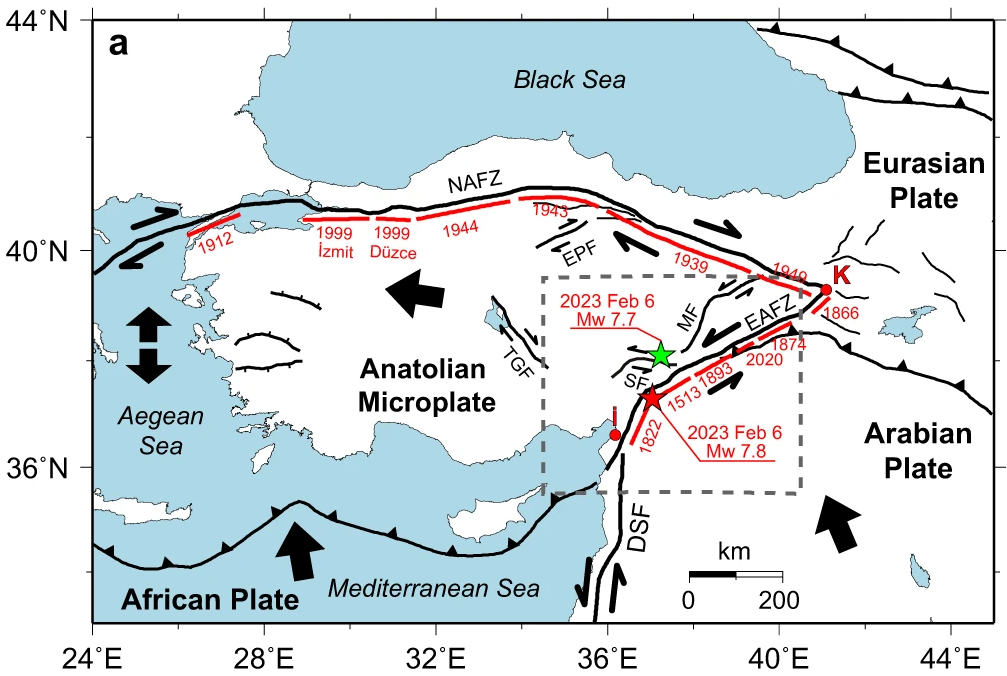
\includegraphics[width=.54\textwidth]{figures/eqturk23_tect.png}
  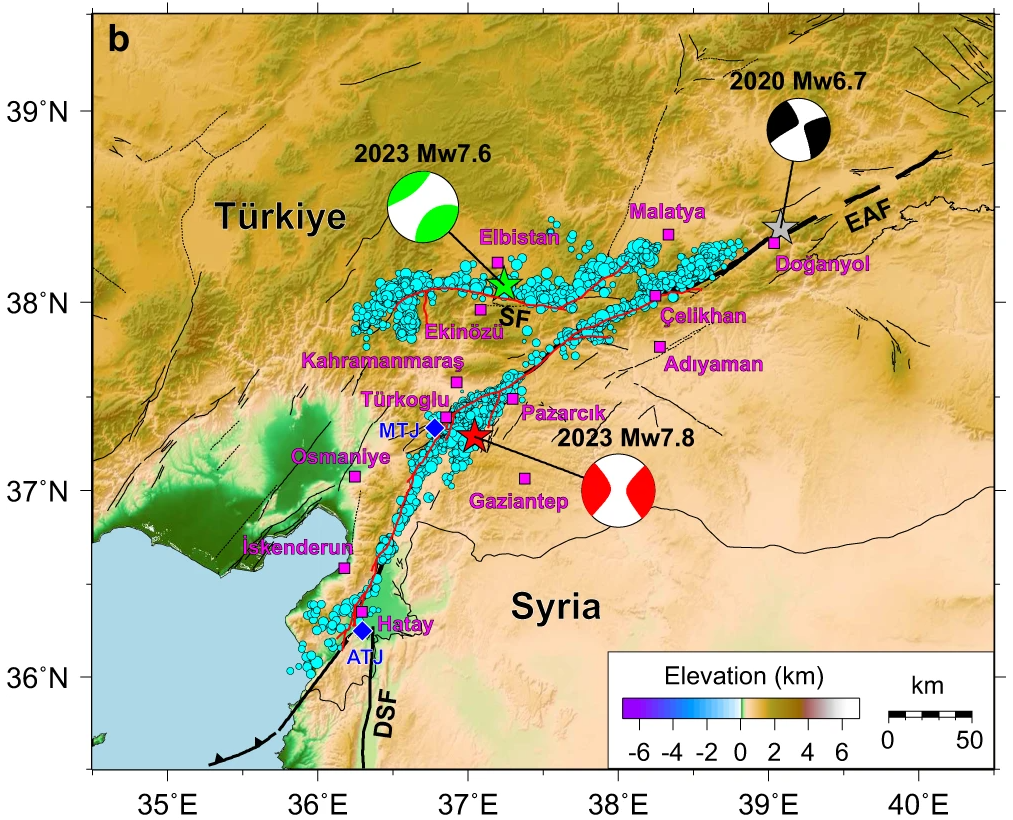
\includegraphics[width=.44\textwidth]{figures/eqturk23_fm.png}\\
%  Fig.1:Tectonic backround (a) and focal mechanisms (b) of 2023 Turkey earthquake doublet
\end{center}
Tectonic backround (a) and focal mechanisms (b) of 2023 Turkey earthquake doublet \cite{Liu_2023}.
%    \label{fig:proc-net}
%\end{figure} 
%\vspace*{-.5cm}


% \vspace{0.3em} % When there are two boxes, some whitespace may need to be added if the one on the right has more content
}




%----------------------------------------------------------------------------------------
%	VELOCITY FIELD
%----------------------------------------------------------------------------------------

\headerbox{Analysis Results}{name=data,column=2, span=2,row=0}{
\label{Analysis_Results}
\begin{minipage}{\textwidth}
\begin{minipage}{0.49\textwidth}
  \begin{center}
    \textbf{Near-field stations}
  \end{center}
\end{minipage}
\begin{minipage}{0.49\textwidth}
  \begin{center}
    \textbf{Far-field stations}
  \end{center}
\end{minipage}

\begin{minipage}{0.24\textwidth}
  \begin{center}
    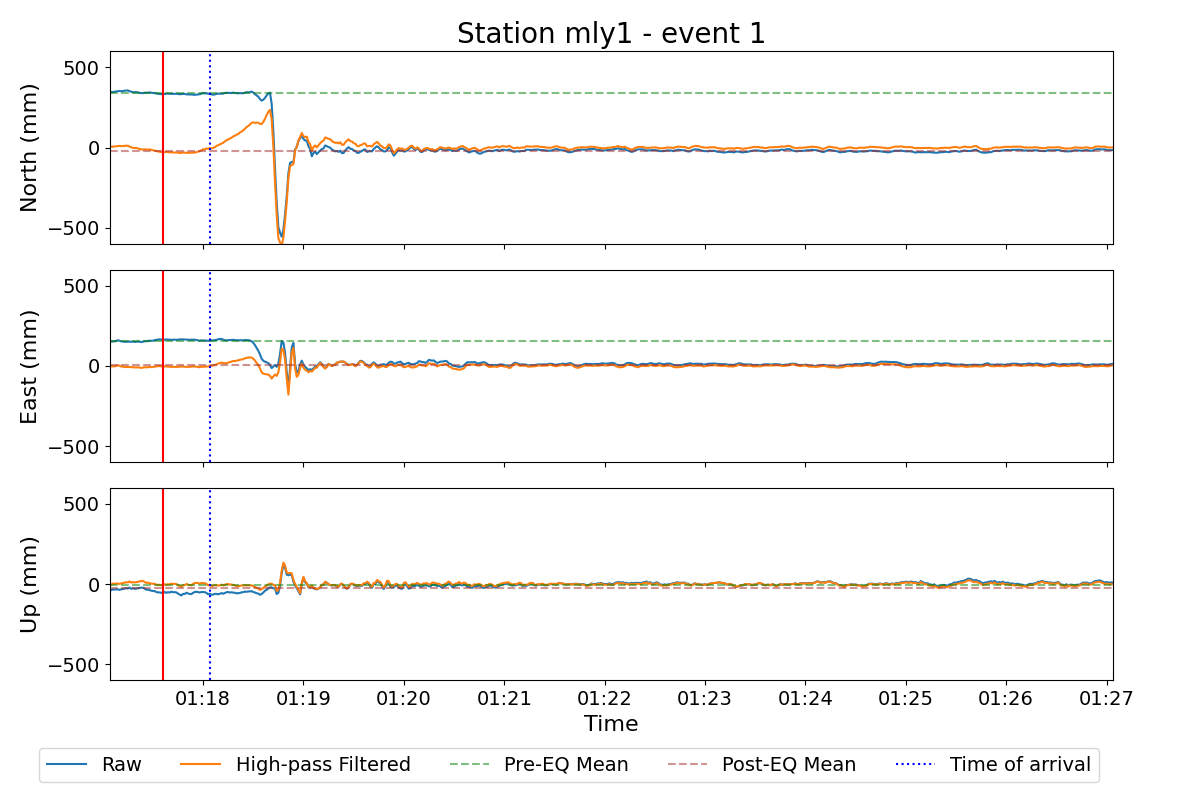
\includegraphics[width=.97\textwidth]{mly1_eq1.png}\\
    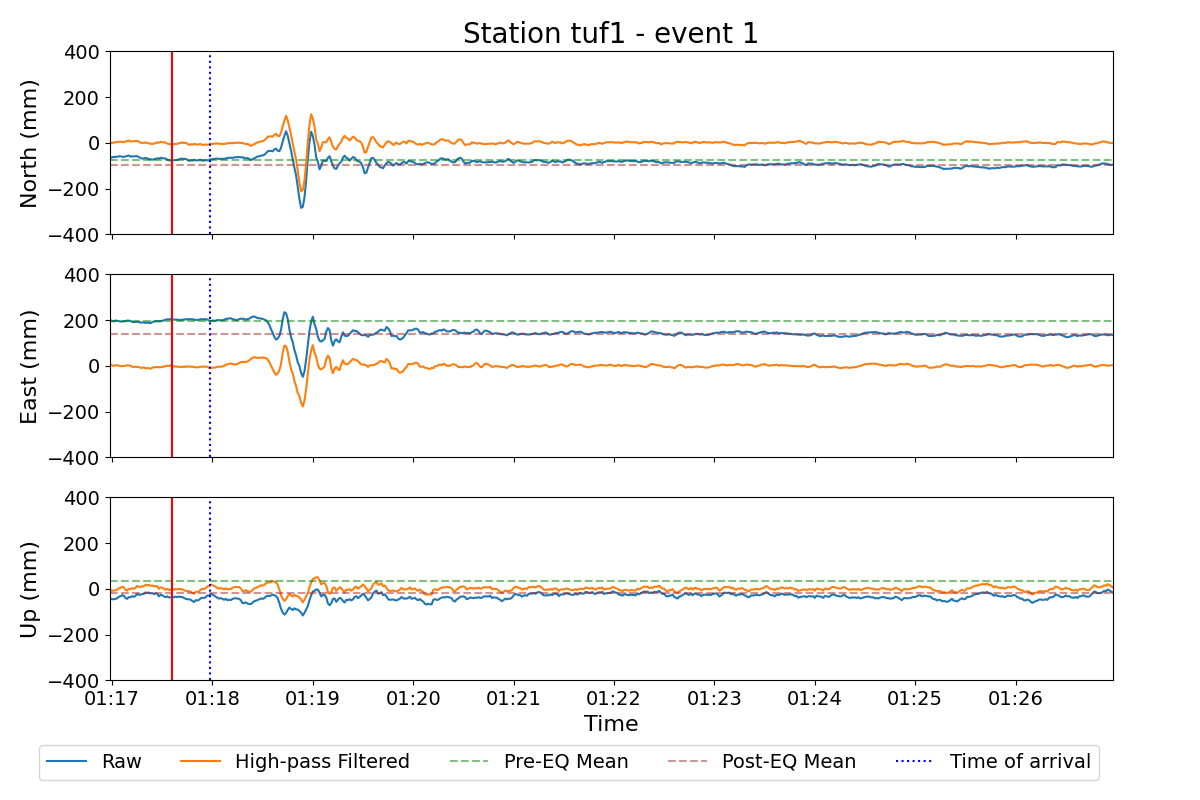
\includegraphics[width=.97\textwidth]{tuf1_eq1.png}\\
    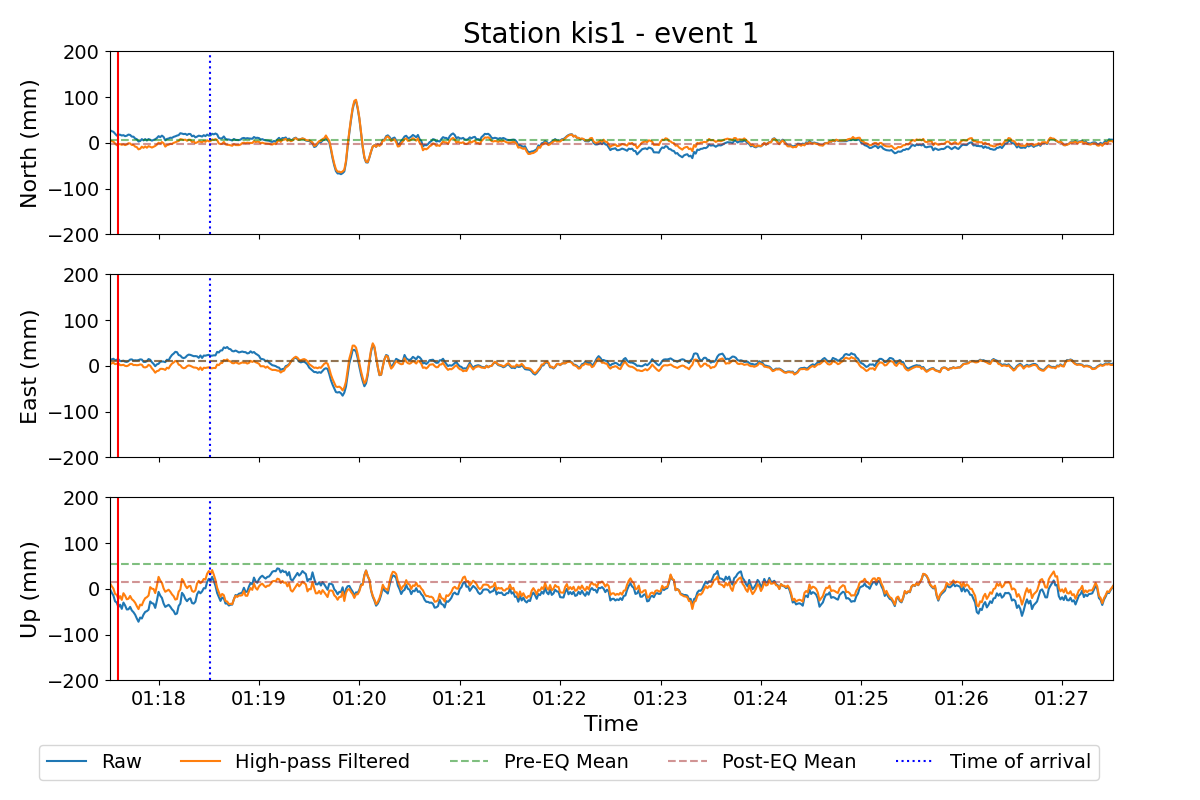
\includegraphics[width=.97\textwidth]{kis1_eq1.png}\\
    %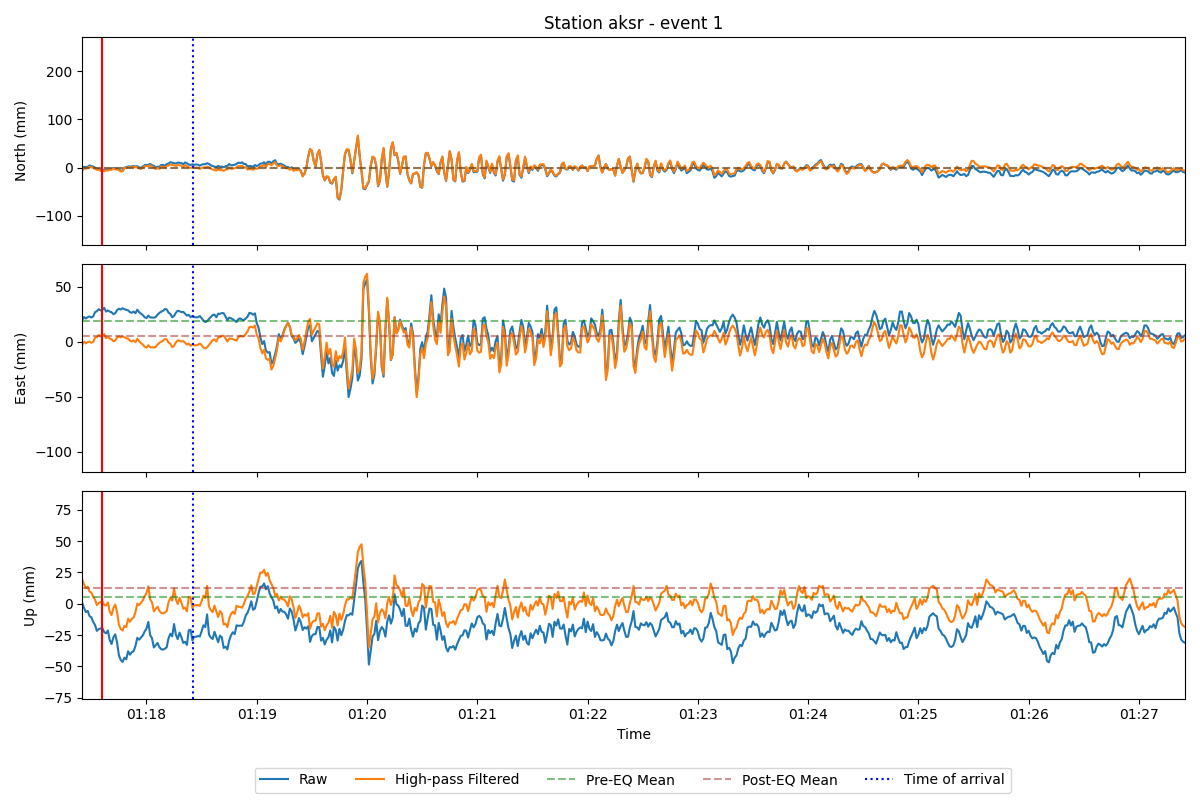
\includegraphics[width=.97\textwidth]{aksr_eq1.png}\\
  \end{center}
\end{minipage}
\begin{minipage}{0.24\textwidth}
  \begin{center}
    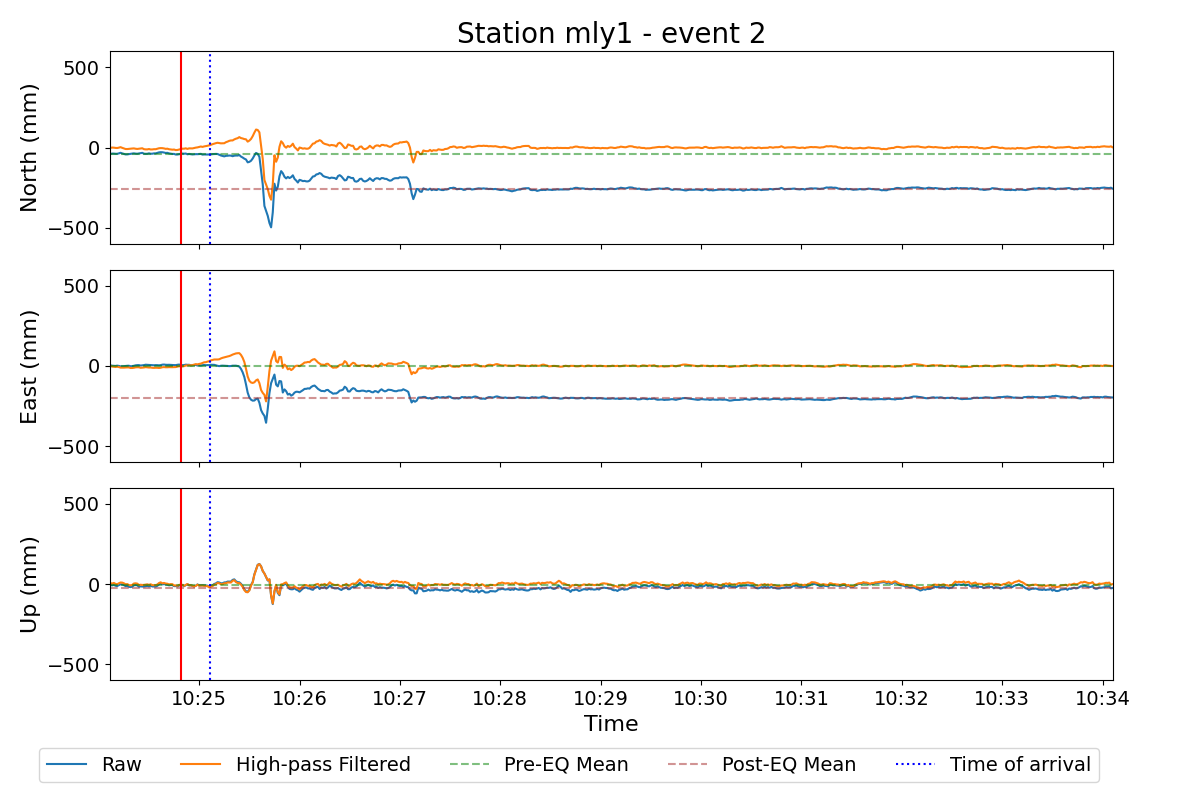
\includegraphics[width=.97\textwidth]{mly1_eq2.png}\\
    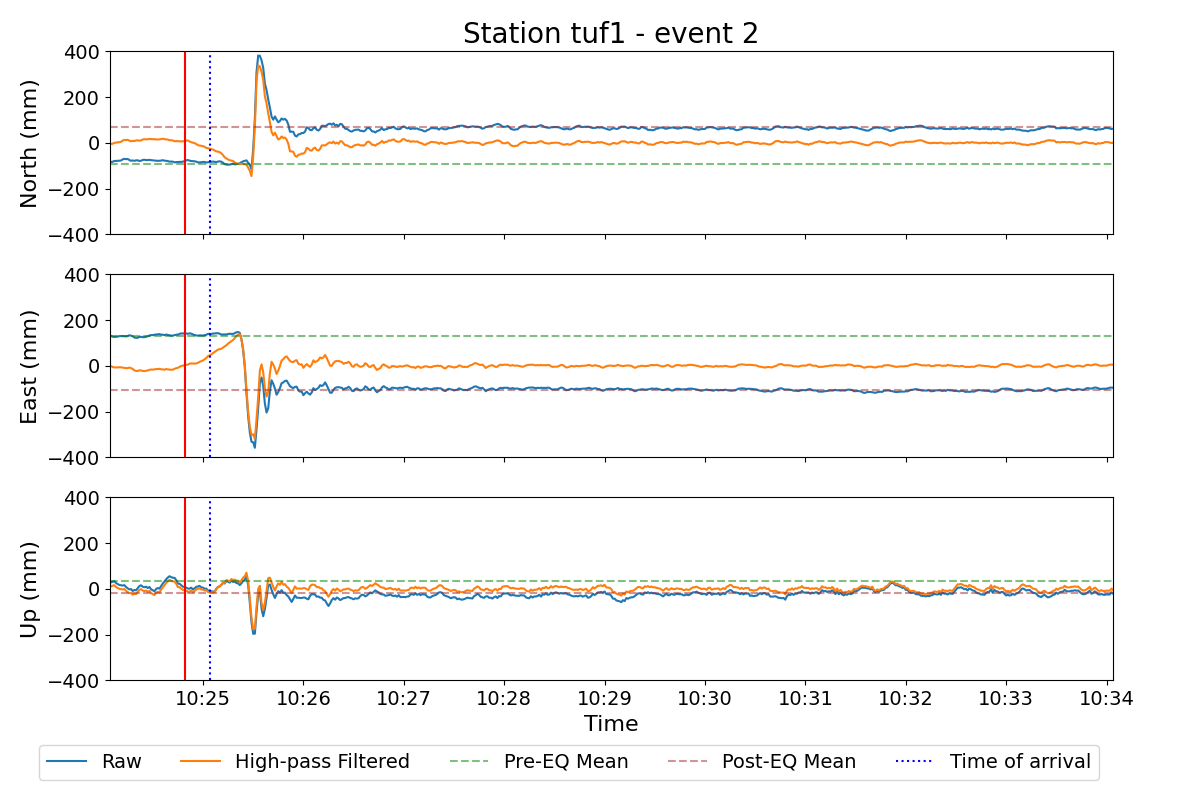
\includegraphics[width=.97\textwidth]{tuf1_eq2.png}\\
    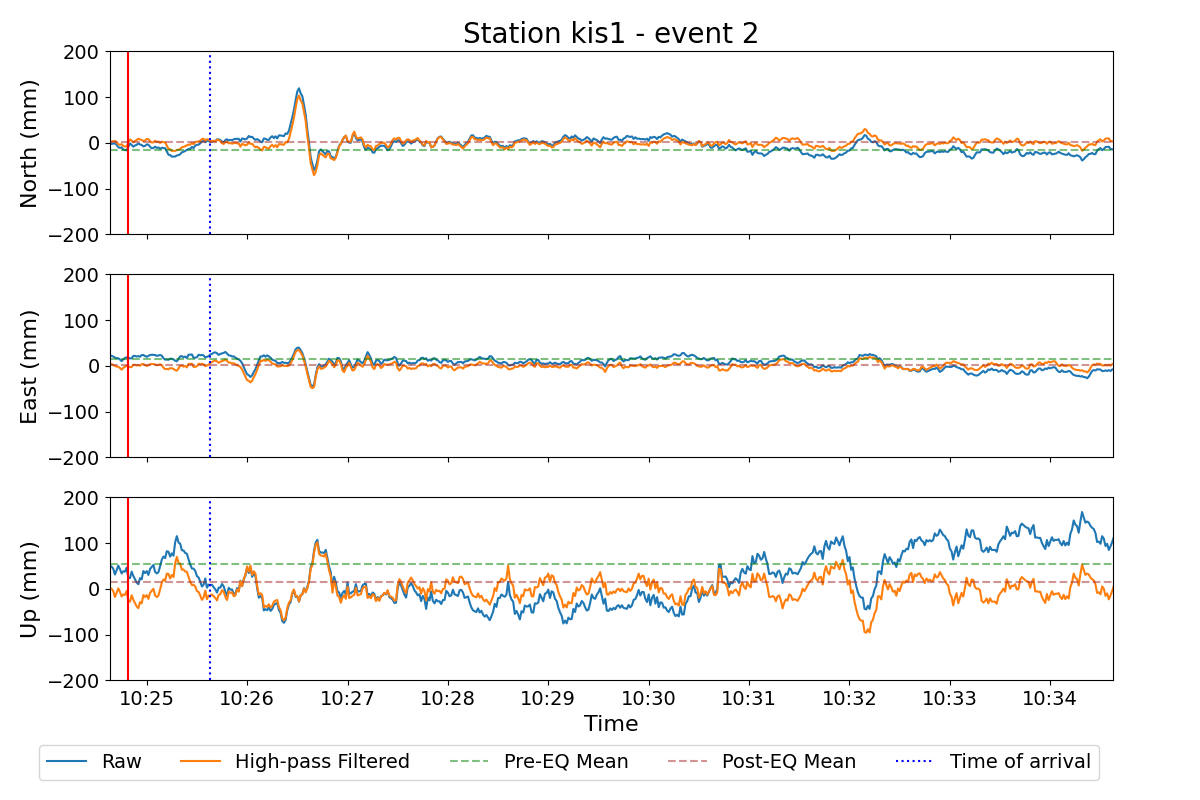
\includegraphics[width=.97\textwidth]{kis1_eq2.png}\\
   % 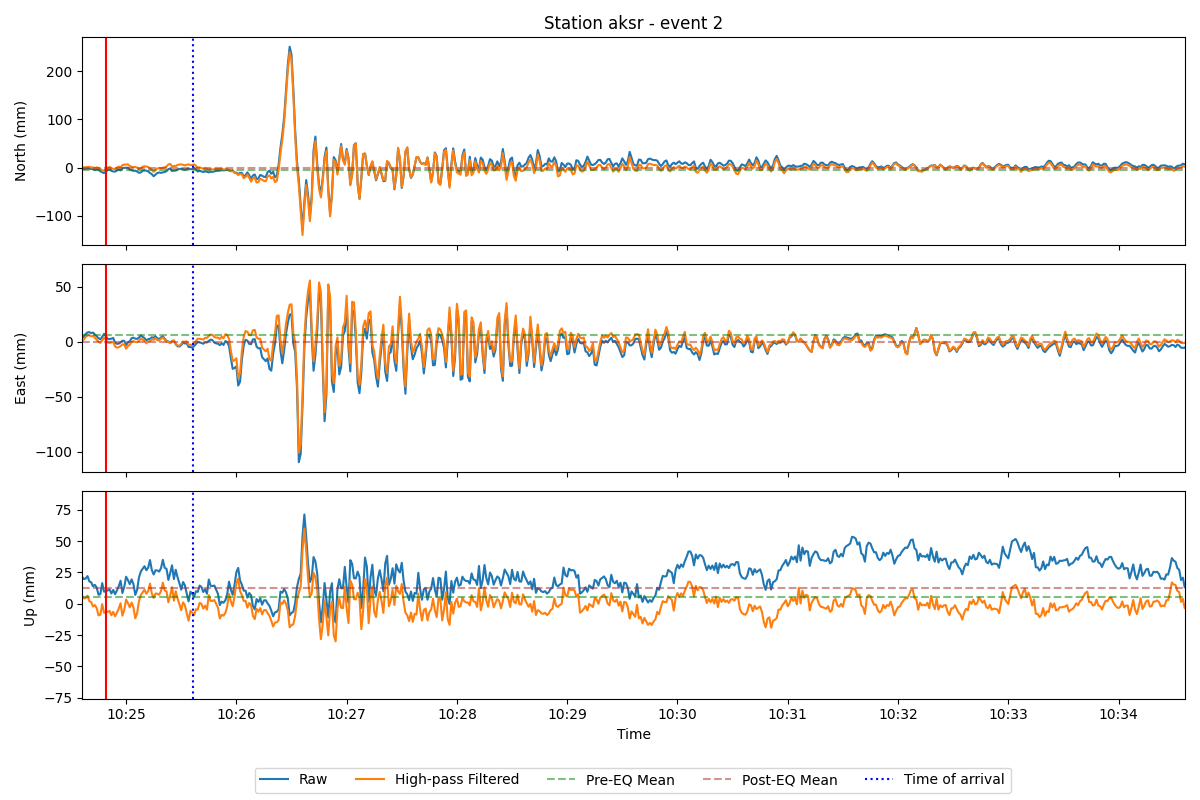
\includegraphics[width=.97\textwidth]{aksr_eq2.png}\\
  \end{center}
\end{minipage}
\textcolor{blue!40}{\vrule width 1pt}
\begin{minipage}{0.24\textwidth}
  \begin{center}
    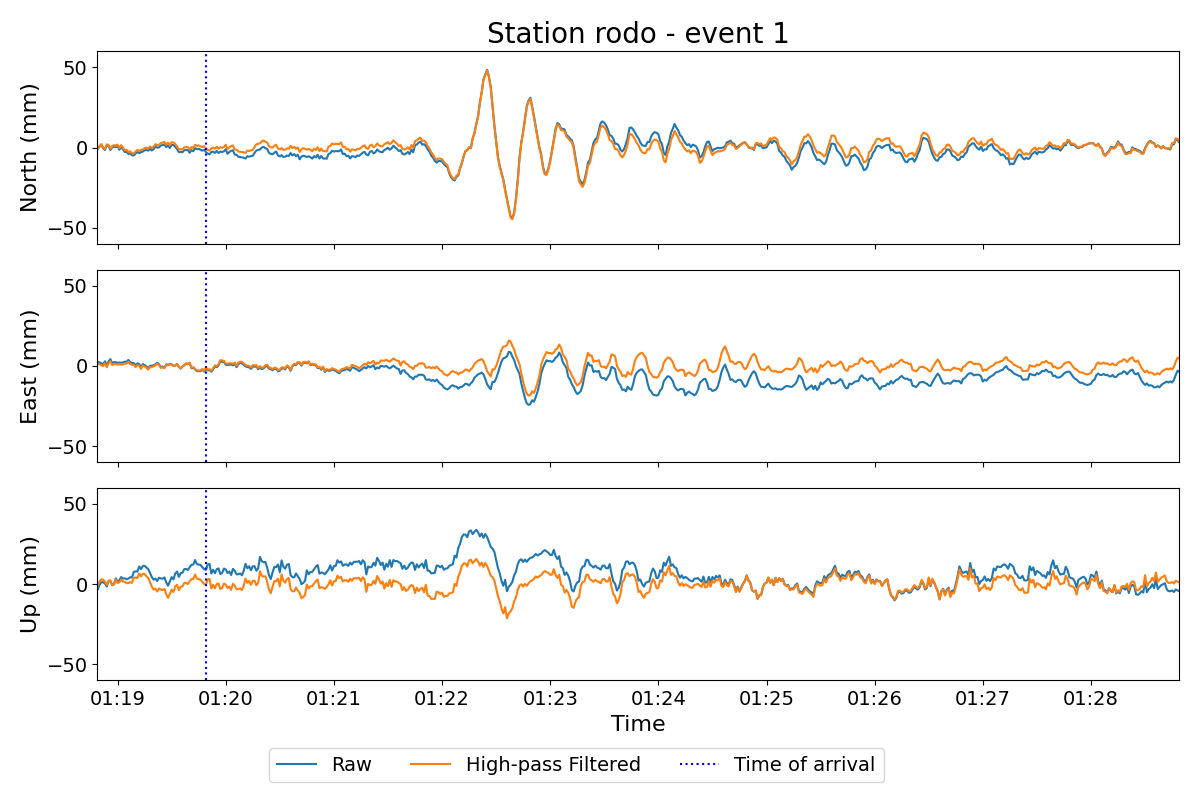
\includegraphics[width=.97\textwidth]{rodo_eq1.png}\\
    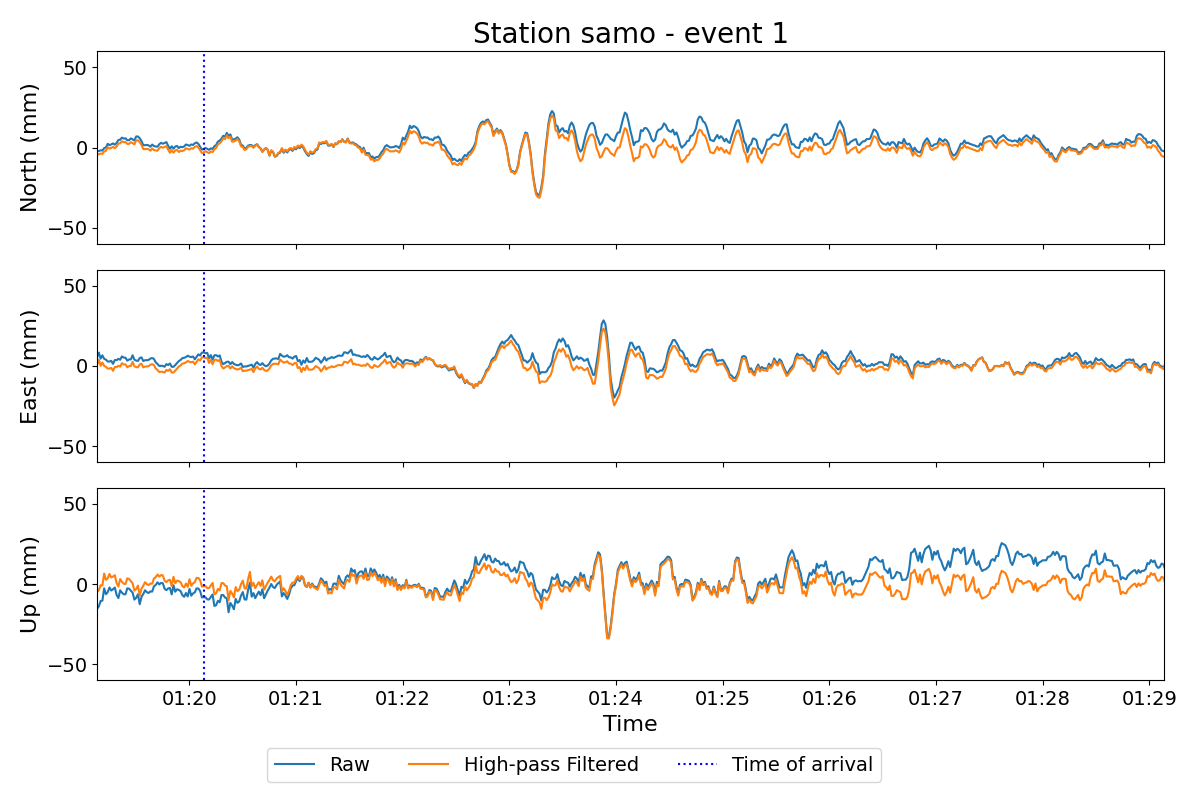
\includegraphics[width=.97\textwidth]{samo_eq1.png}\\
    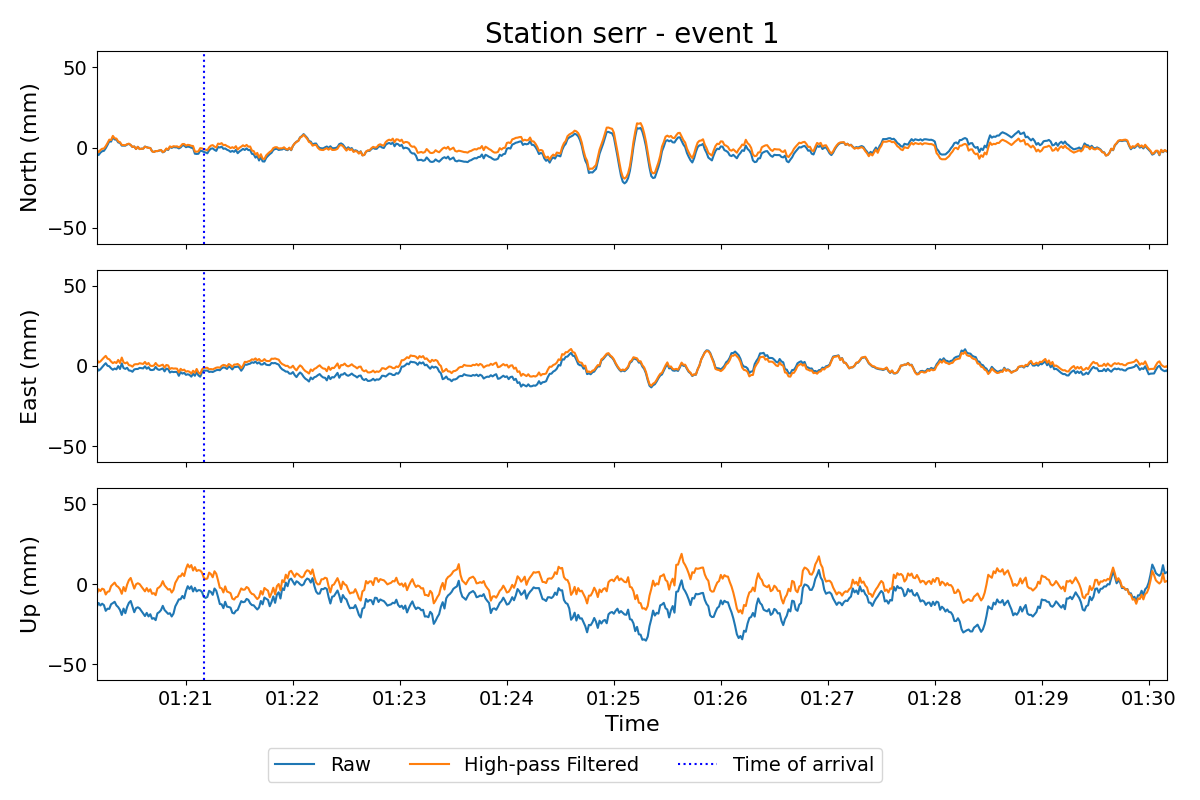
\includegraphics[width=.97\textwidth]{serr_eq1.png}\\
    %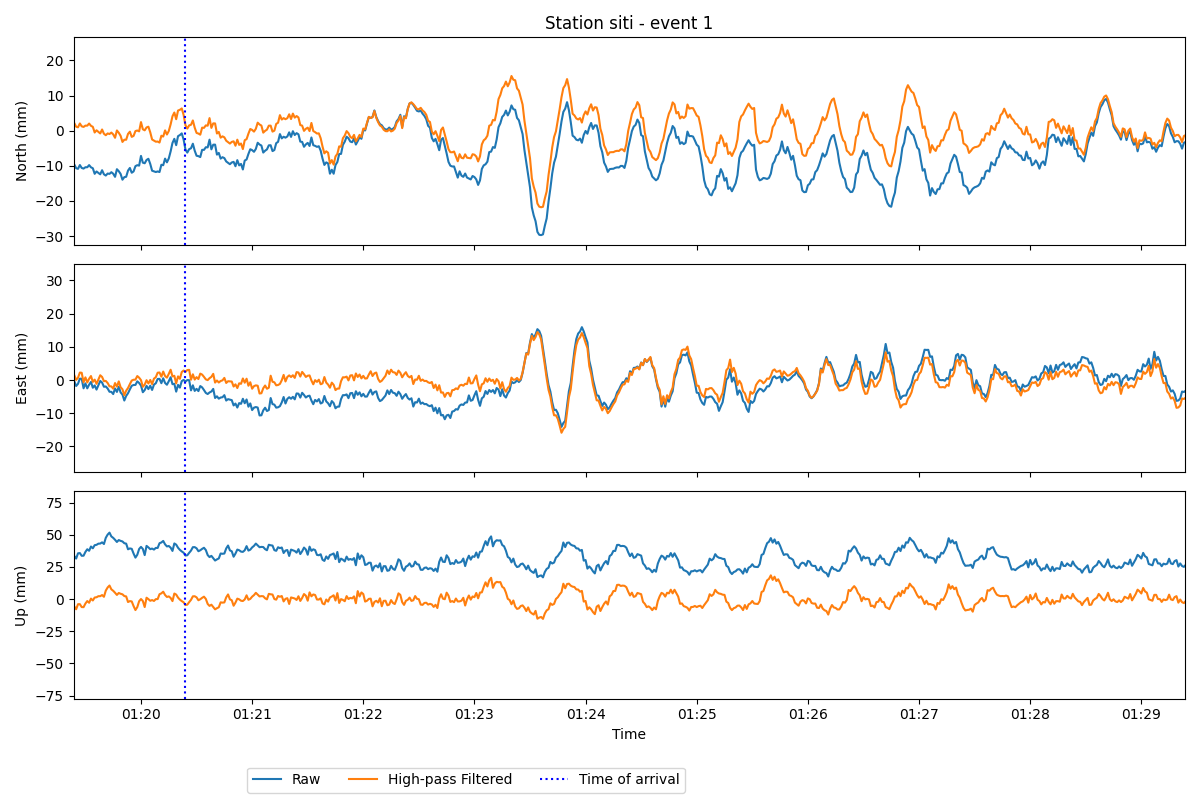
\includegraphics[width=.97\textwidth]{siti_eq1.png}\\
  \end{center}
\end{minipage}
\begin{minipage}{0.24\textwidth}
  \begin{center}
    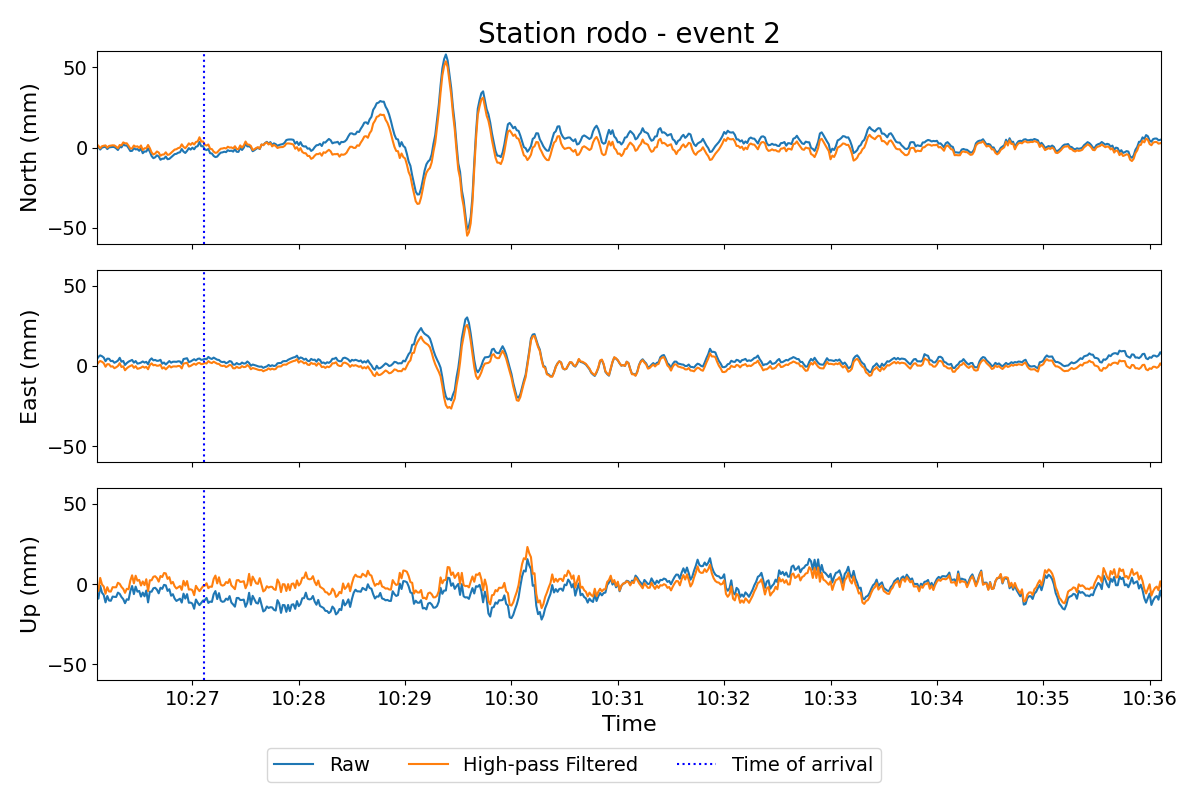
\includegraphics[width=.97\textwidth]{rodo_eq2.png}\\
    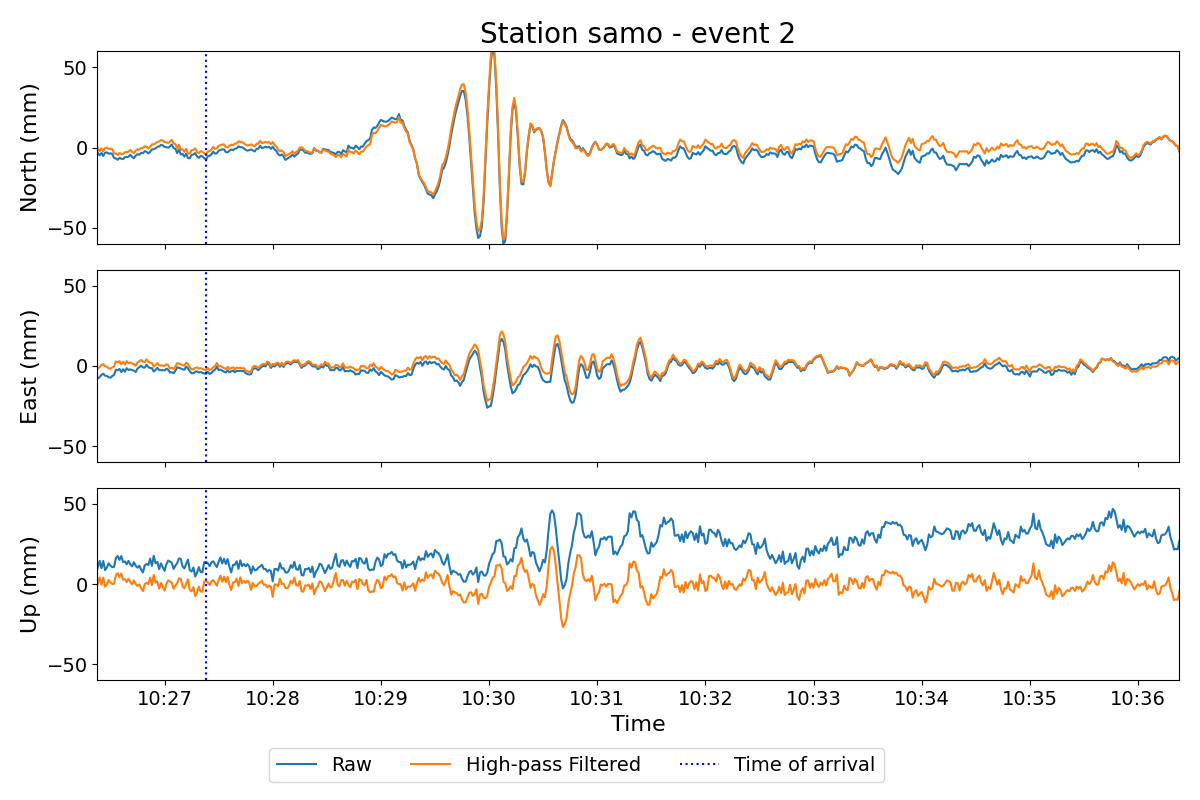
\includegraphics[width=.97\textwidth]{samo_eq2.png}\\
    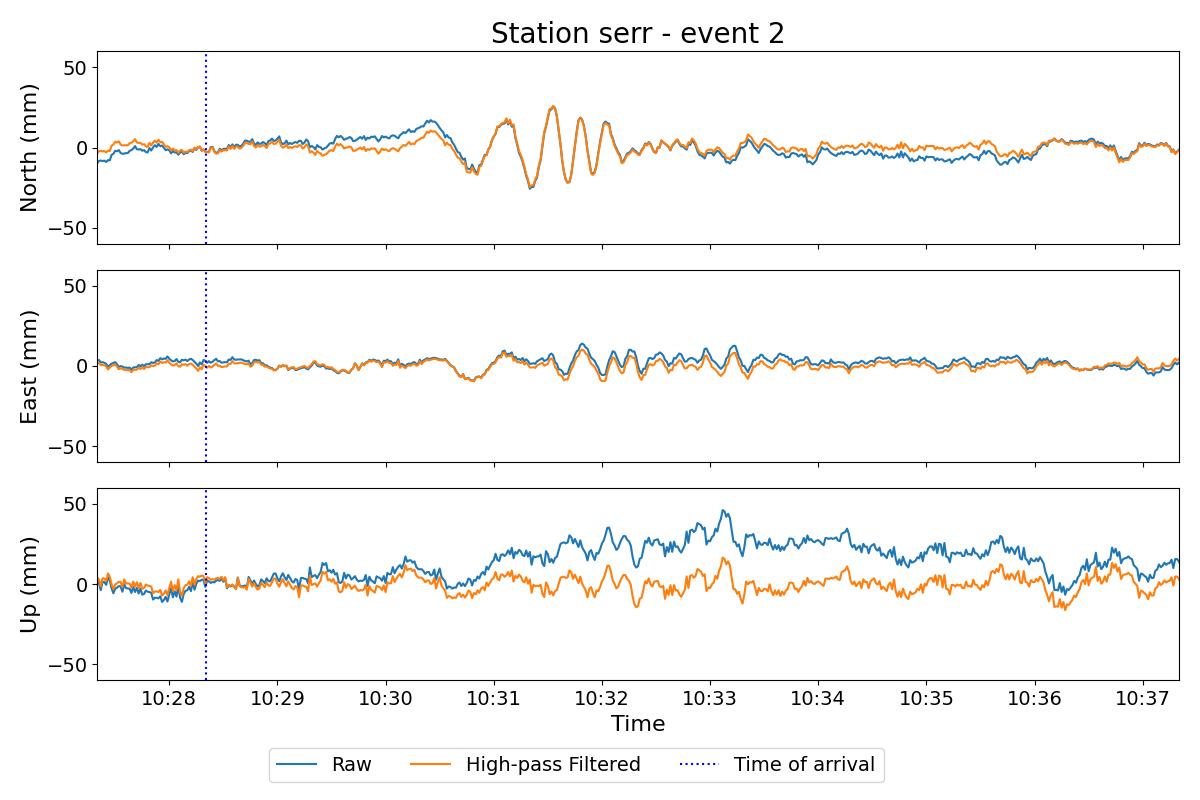
\includegraphics[width=.97\textwidth]{serr_eq2.png}\\
    %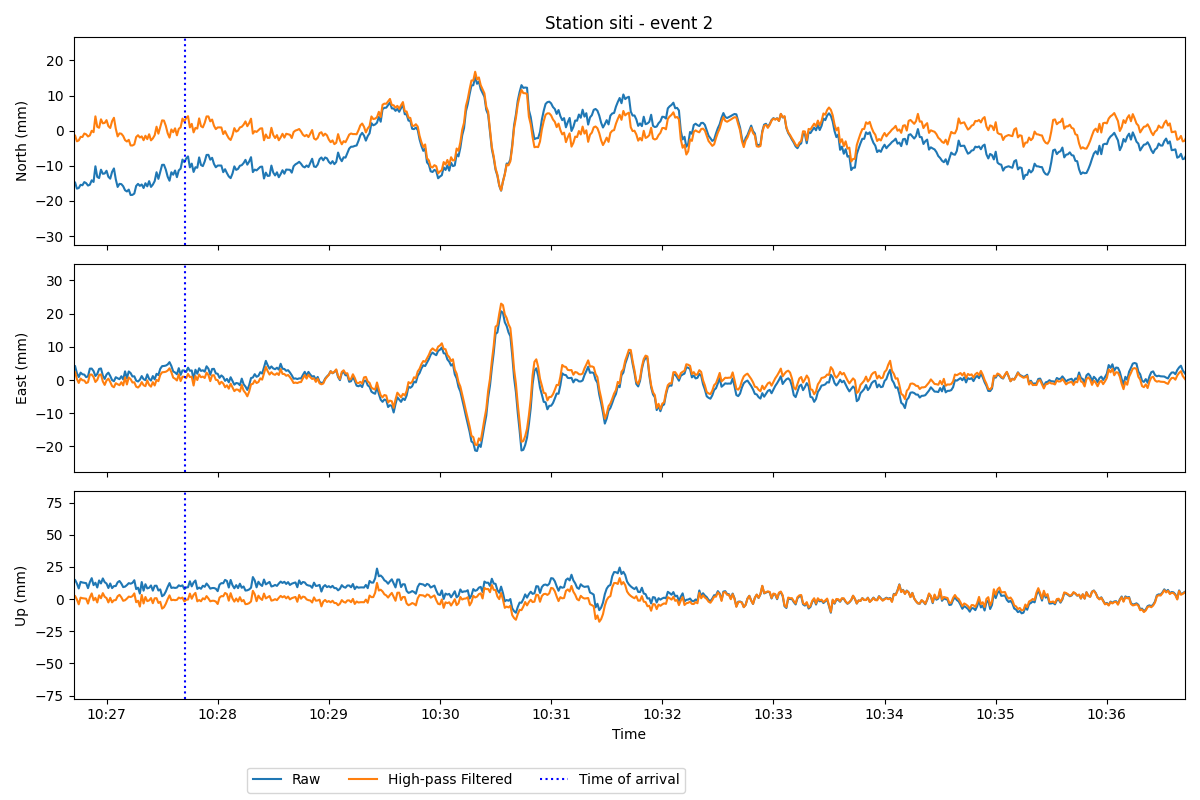
\includegraphics[width=.97\textwidth]{siti_eq2.png}\\
  \end{center}
\end{minipage}
\end{minipage}
\begin{minipage}{.29\textwidth}

\end{minipage}

%%\vfill
%\rotatebox{90}{\scriptsize ~~~~~~~~~~North}
%  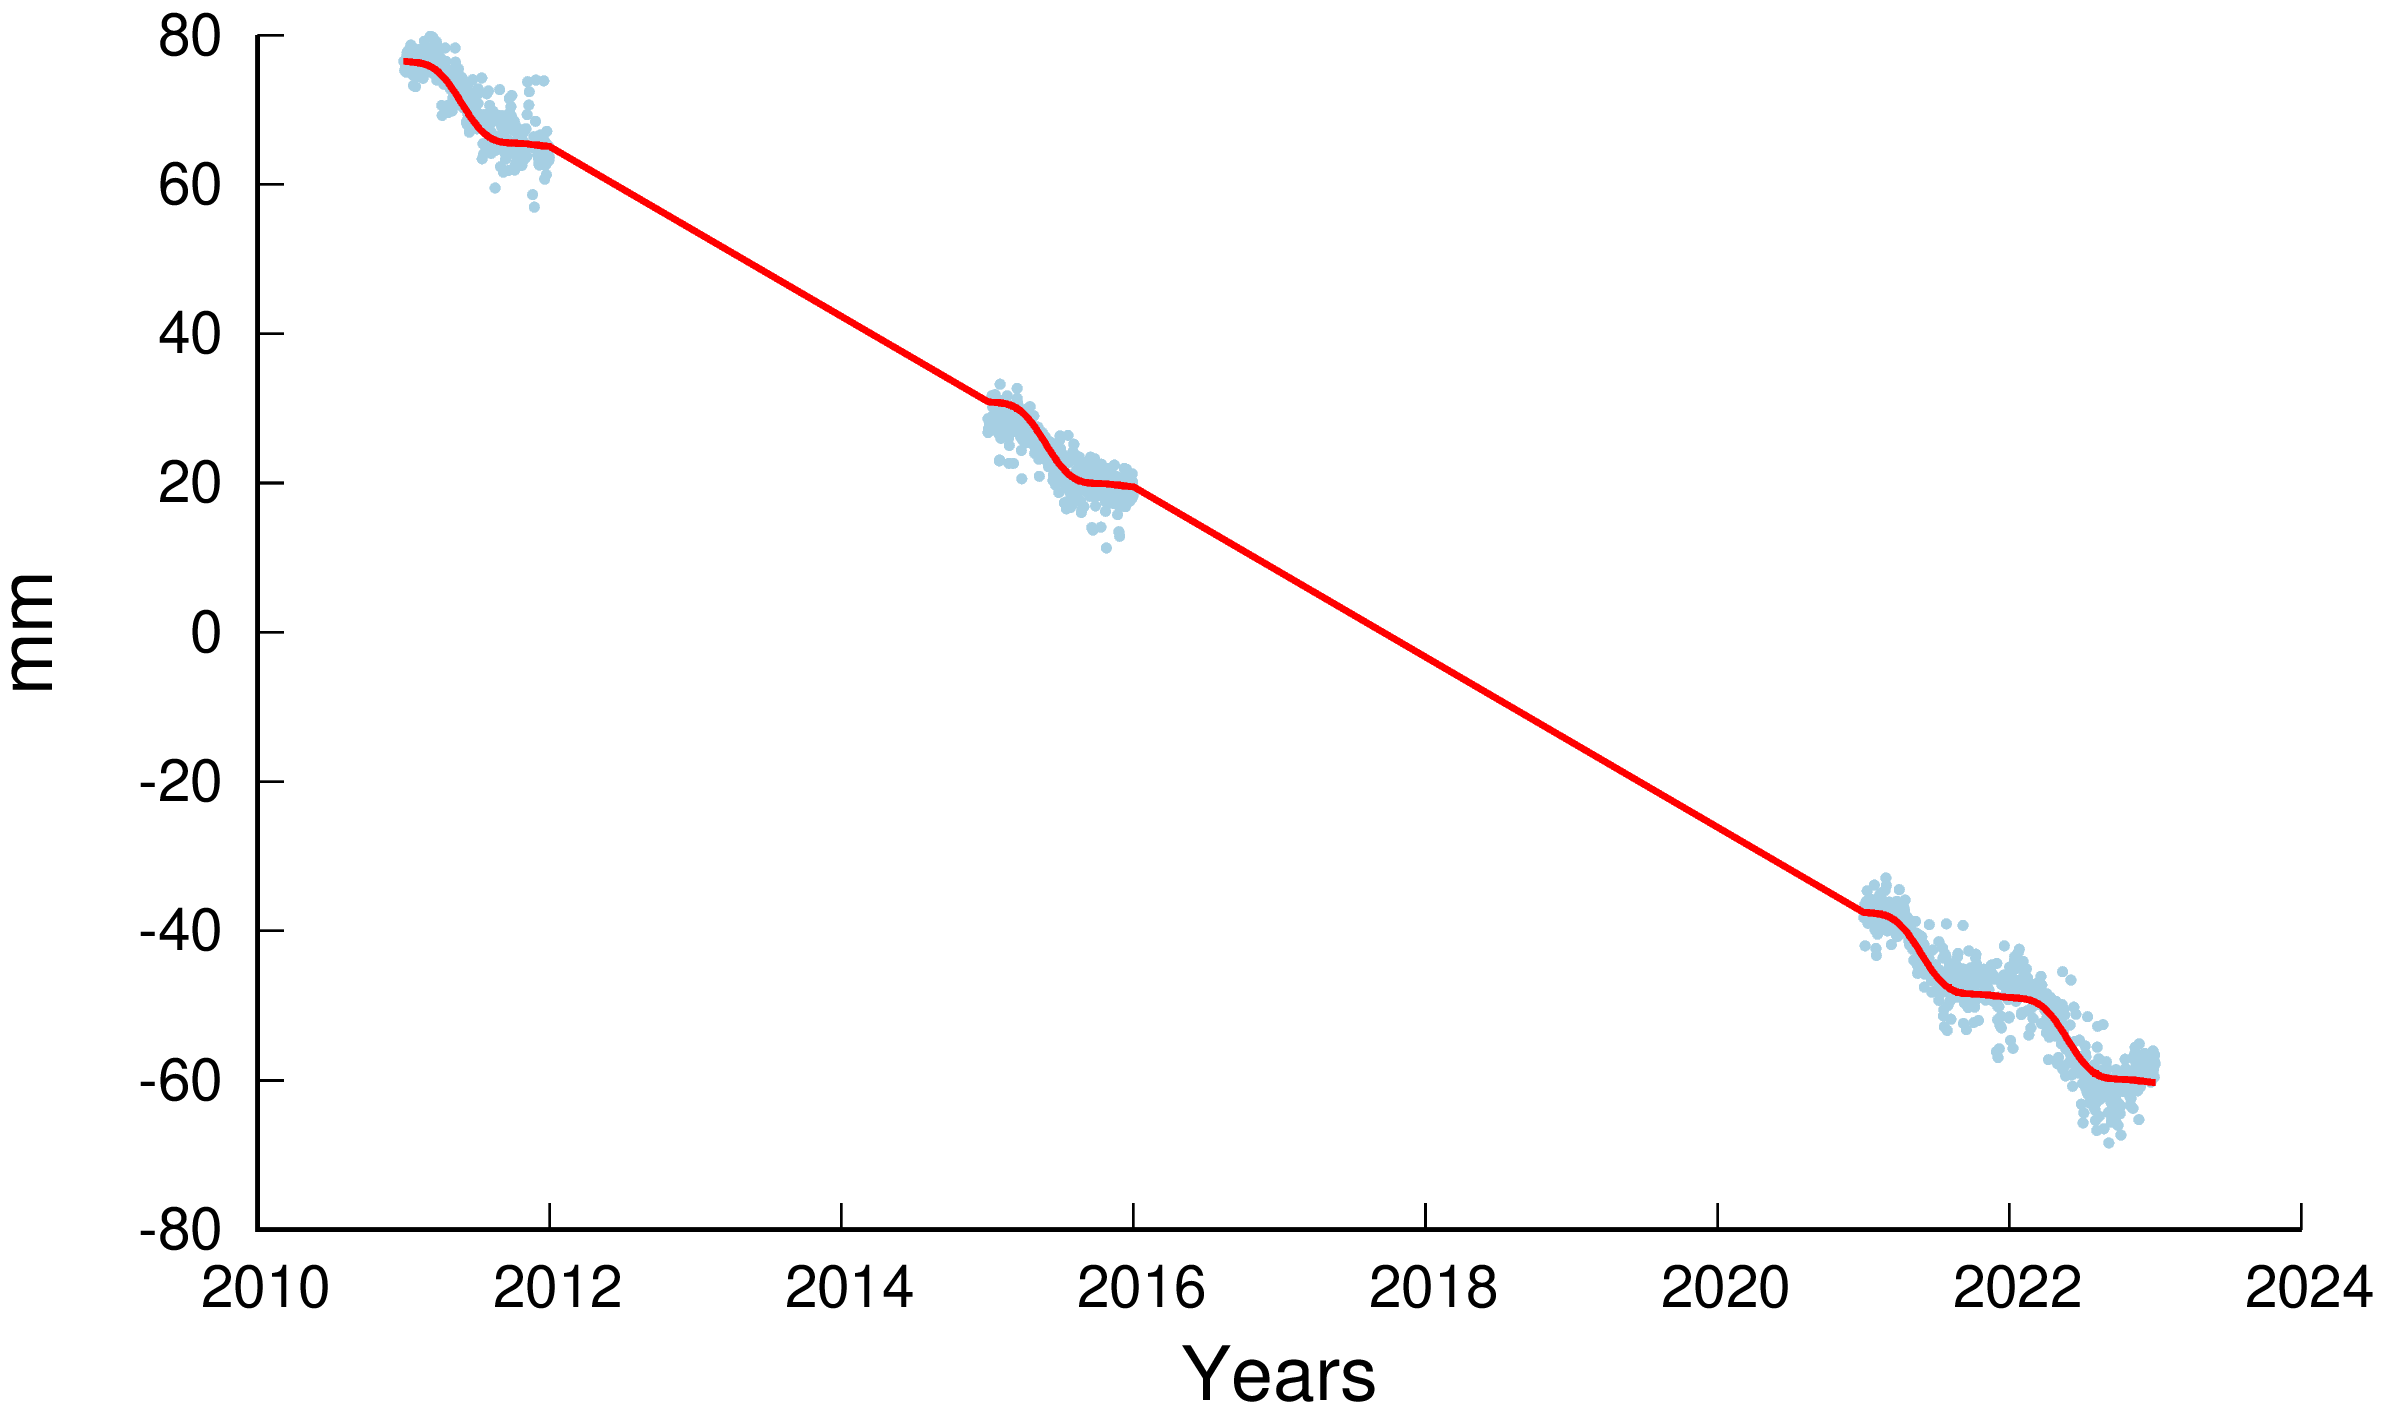
\includegraphics[height=5em]{098a_0_data.png}~
\includegraphics[height=5em]{098a_0_res.png}\\
%\rotatebox{90}{\scriptsize ~~~~~~~~~~~~East}
%  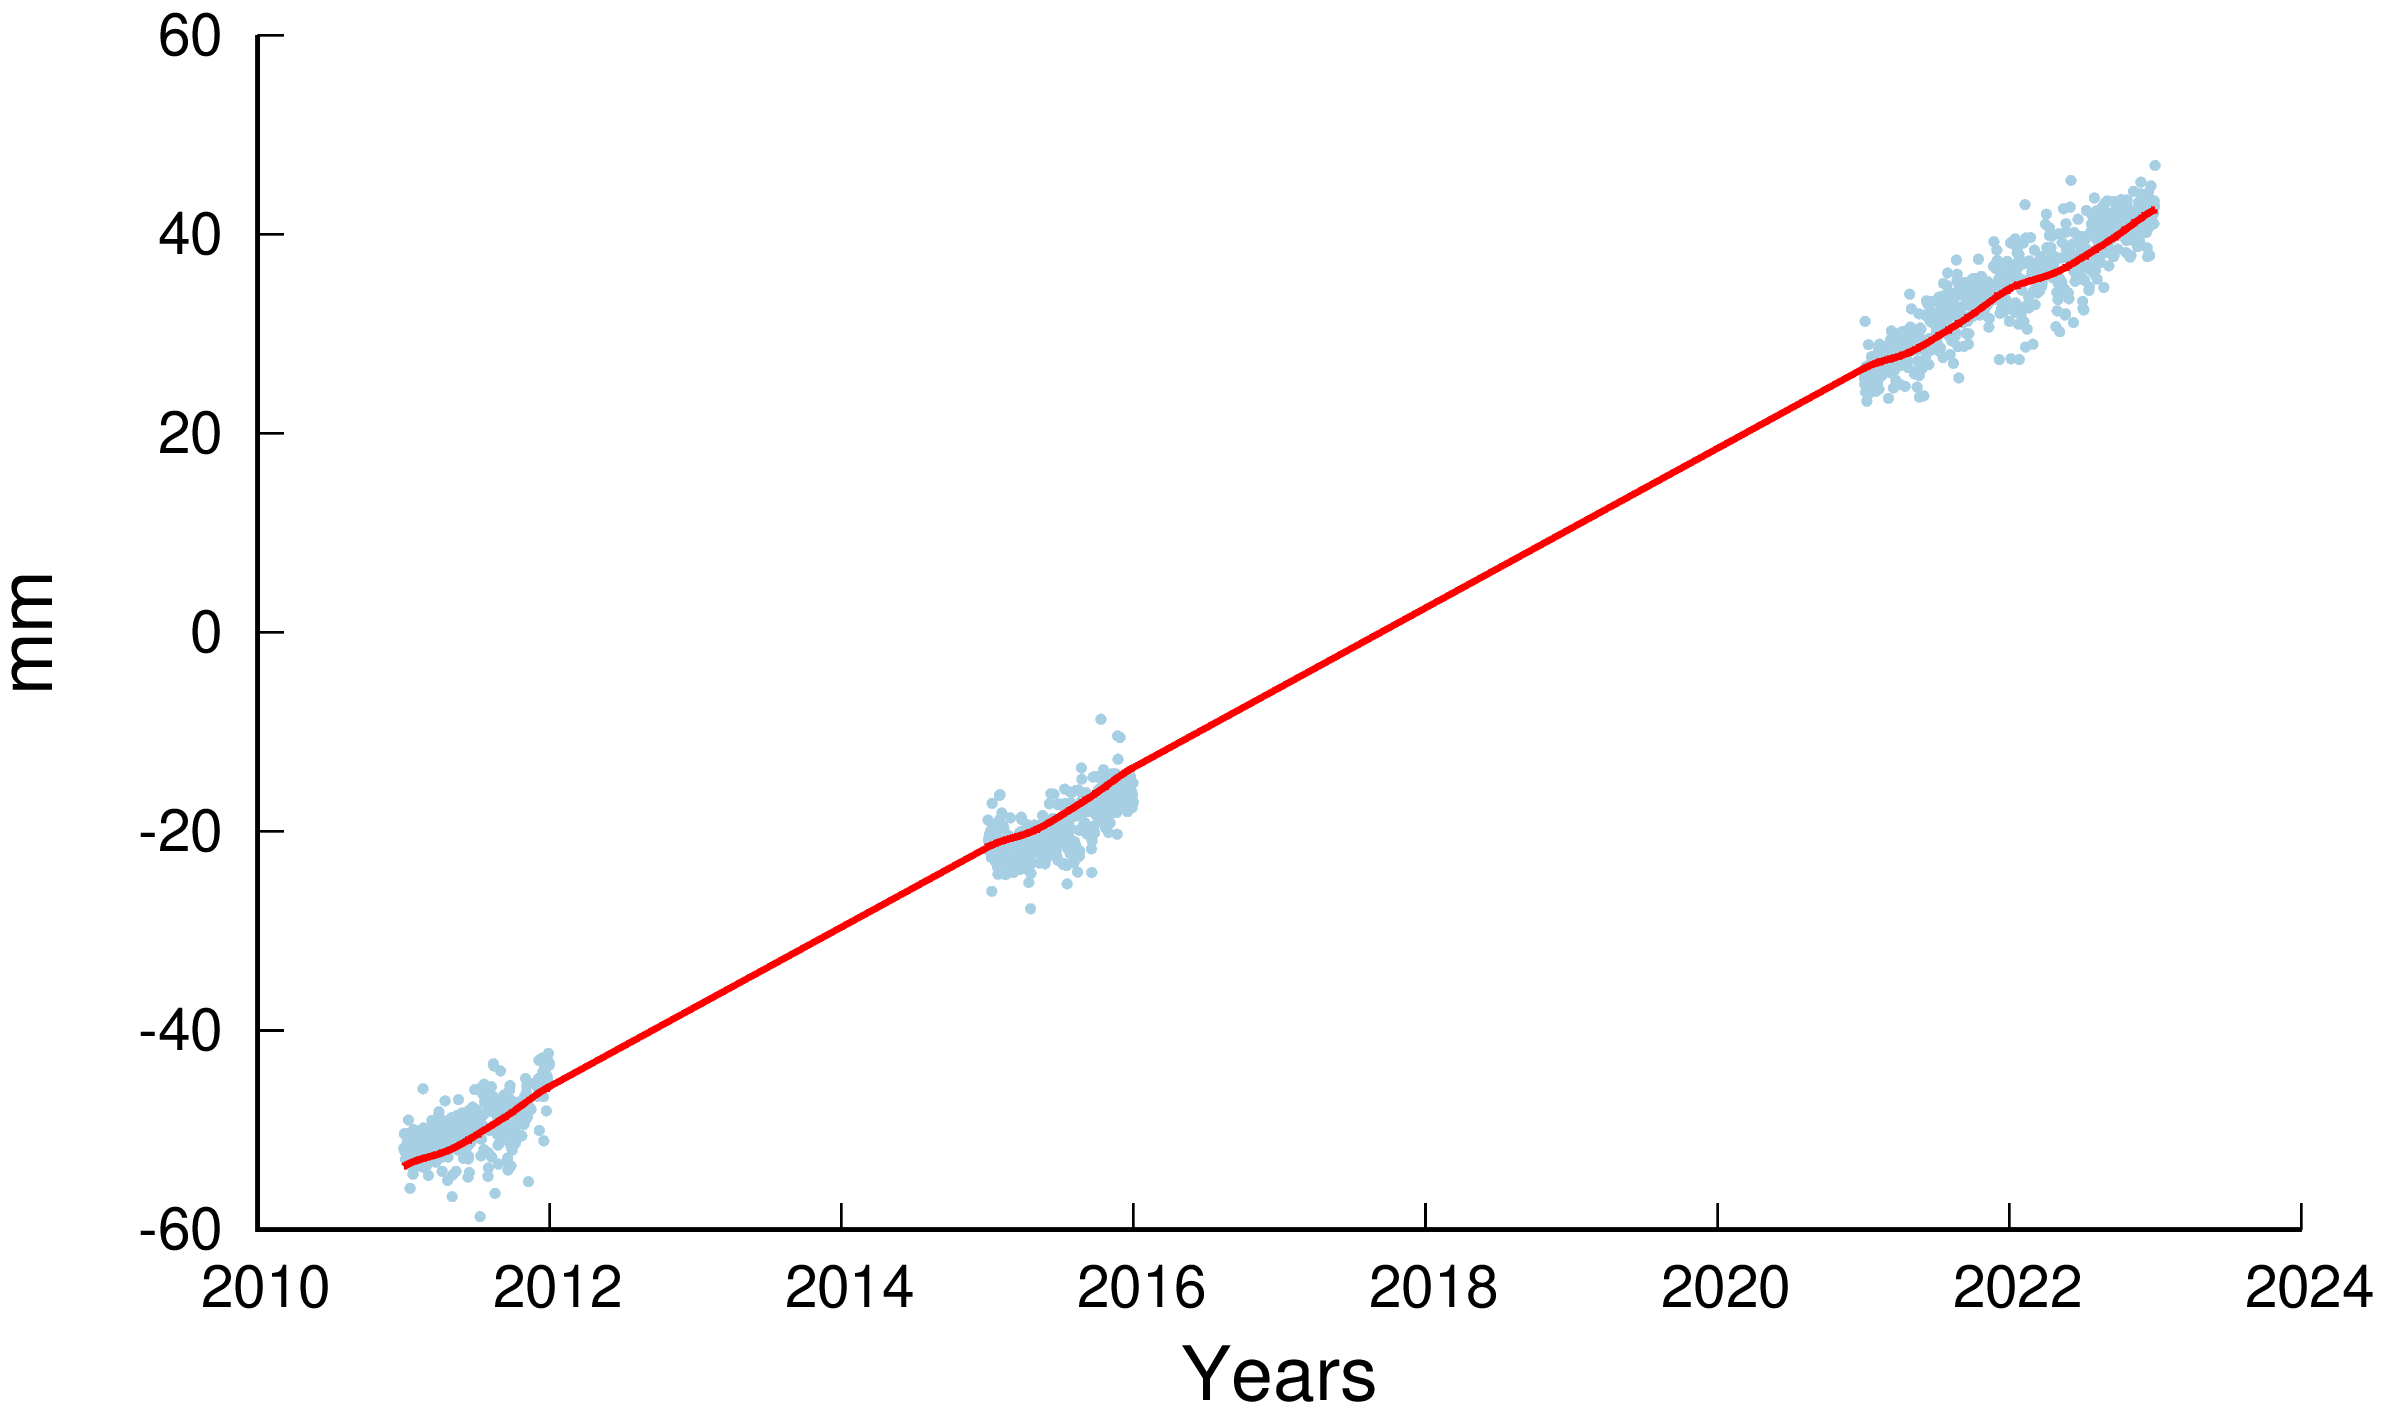
\includegraphics[height=5em]{098a_1_data.png}~
\includegraphics[height=5em]{098a_1_res.png}\\
%\rotatebox{90}{\scriptsize ~~~~~~~~~~~~~~Up}
%  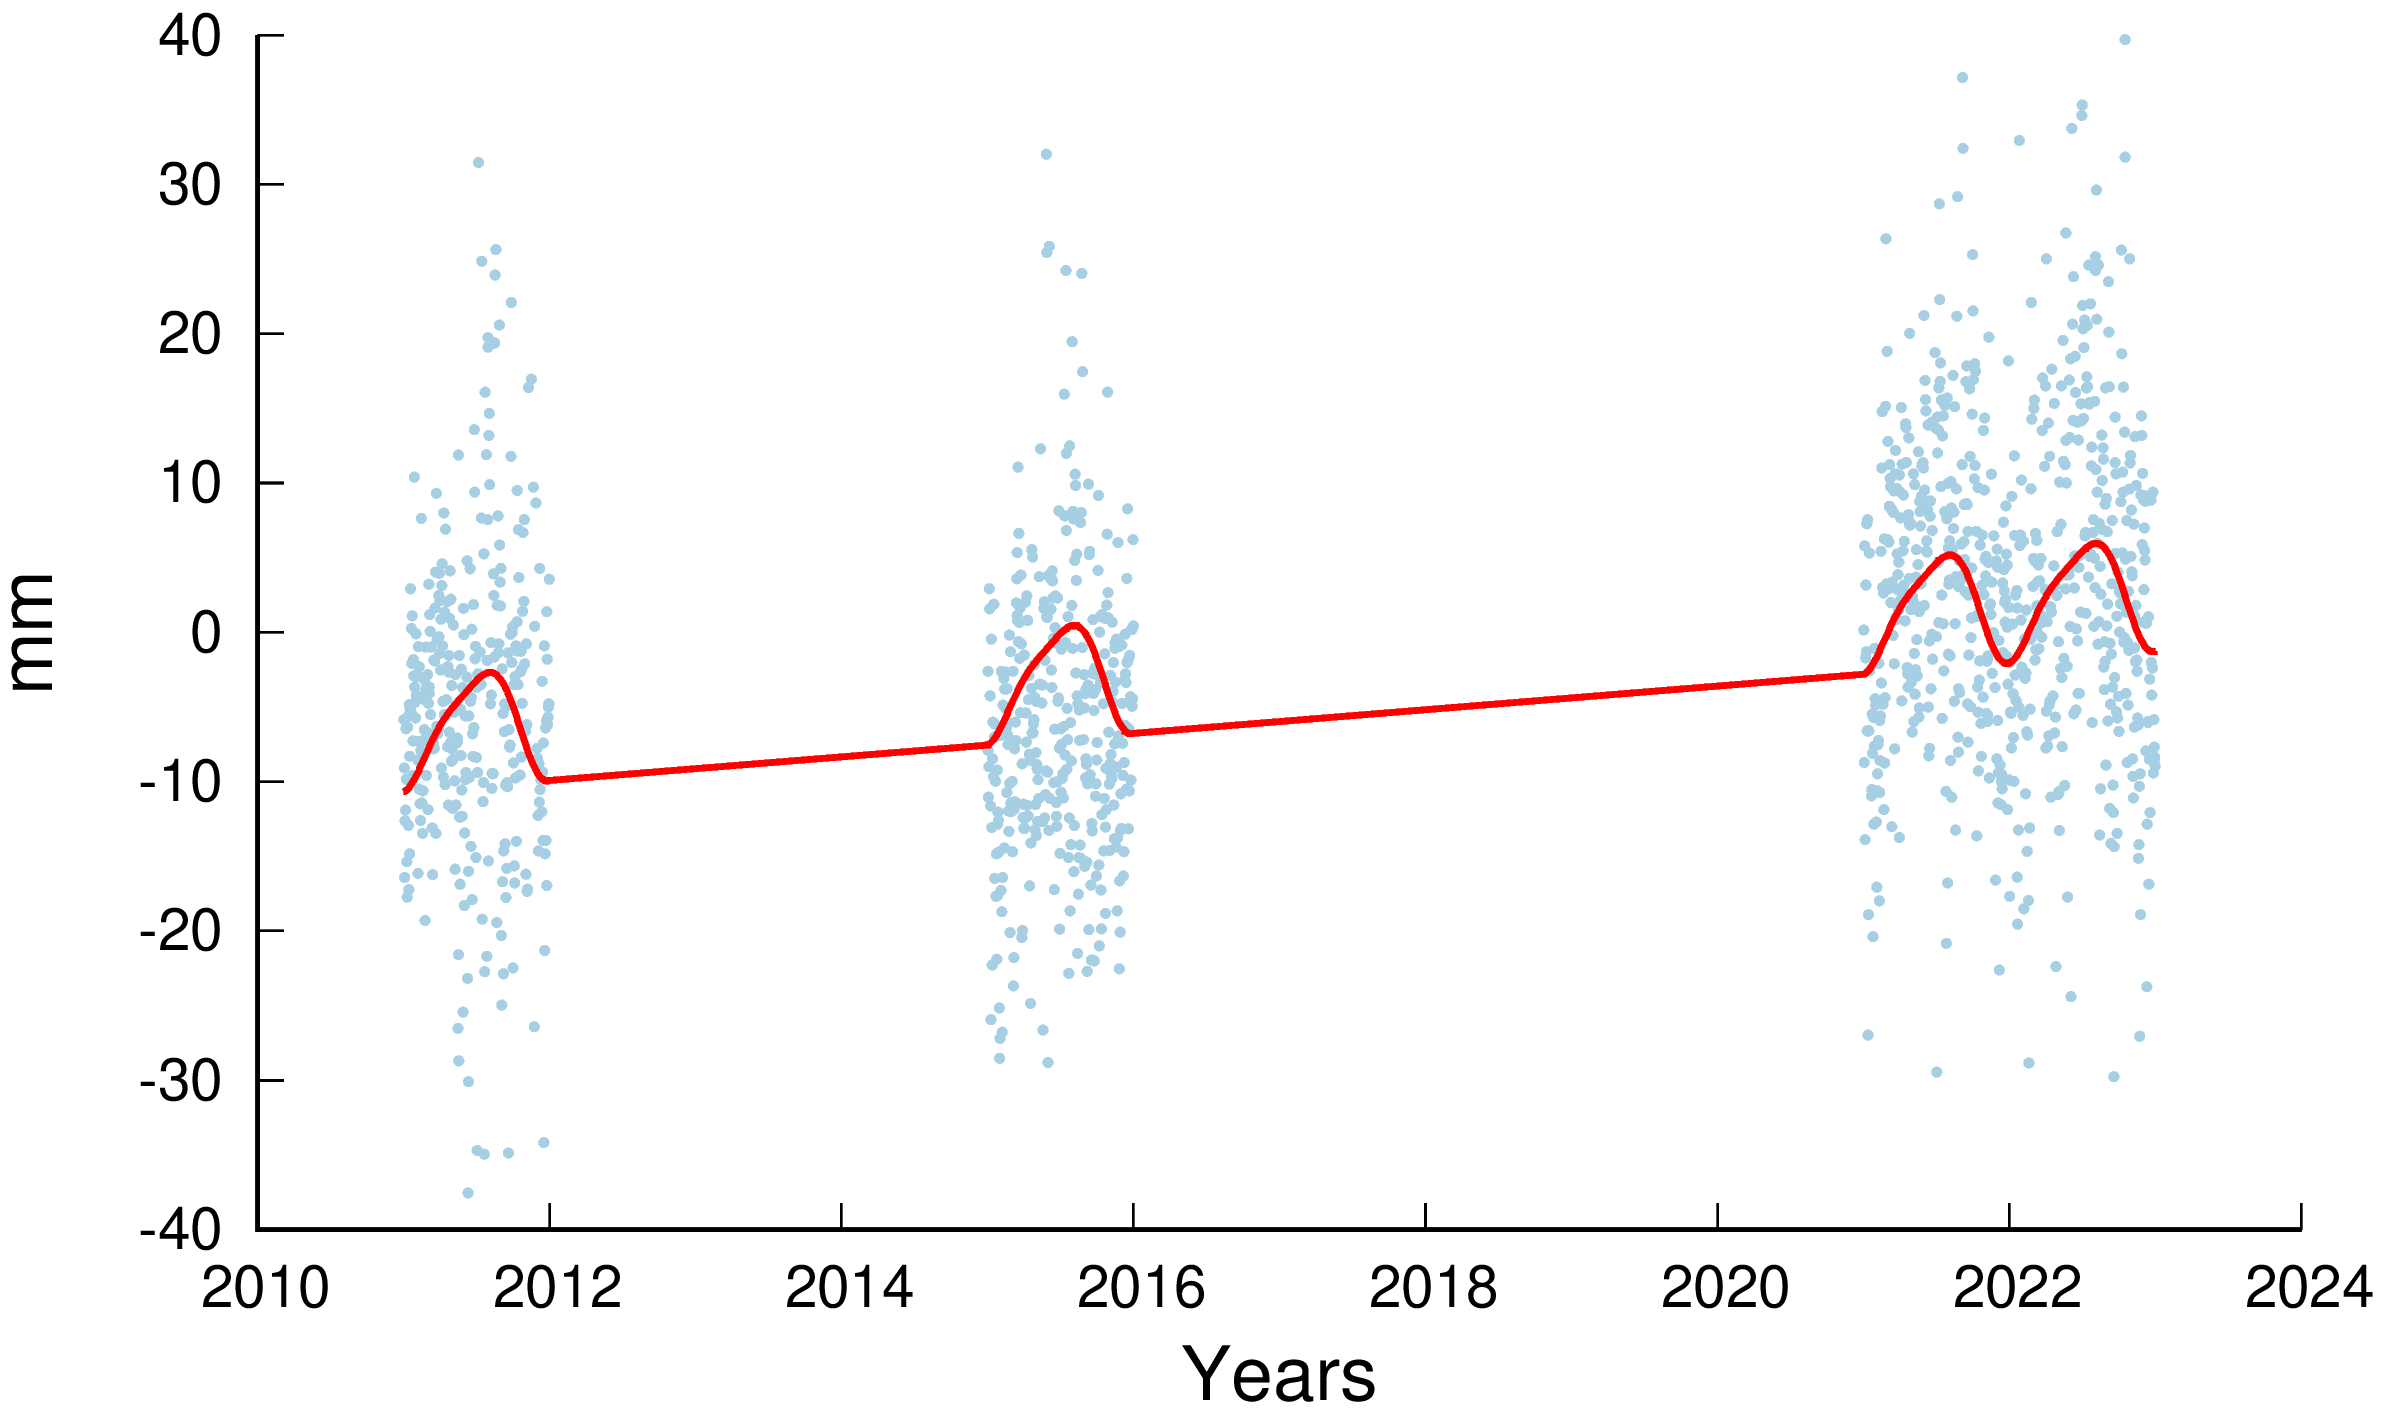
\includegraphics[height=5em]{098a_2_data.png}~
\includegraphics[height=5em]{098a_2_res.png}
%%\vfill
%\end{minipage}
%\begin{minipage}[c]{0.33\linewidth}
%\begin{center}
%057A (co-seismic displacement)
%\end{center}
%  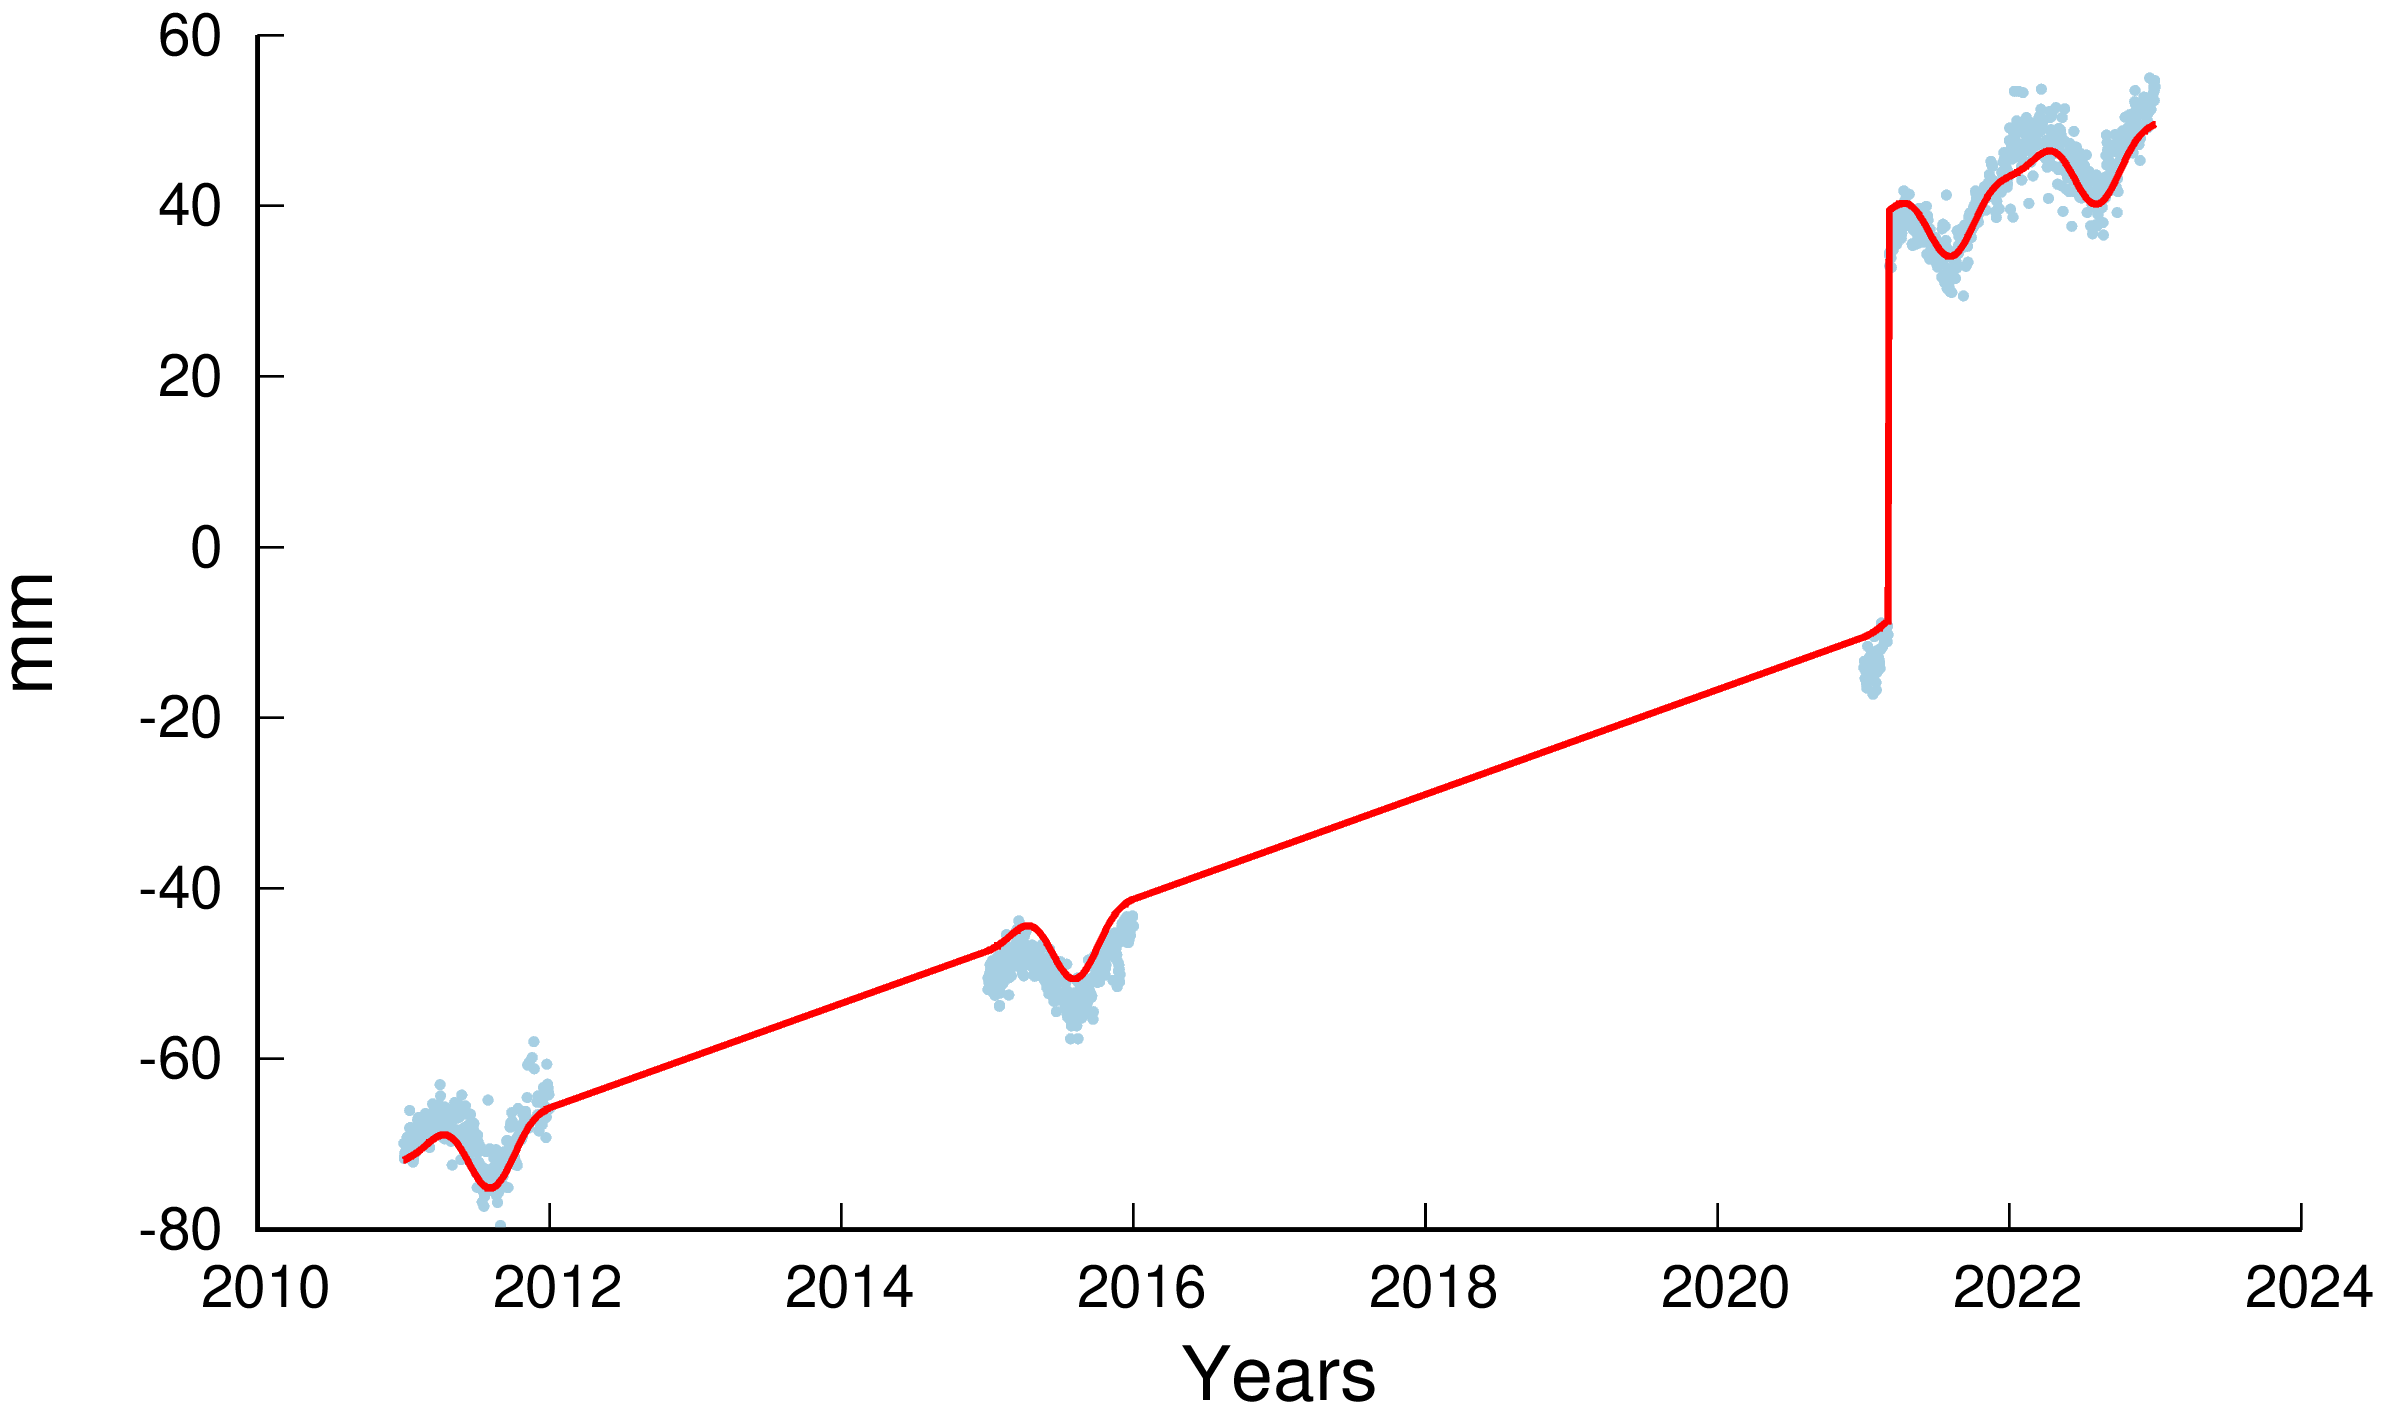
\includegraphics[height=5em]{057a_0_data.png}~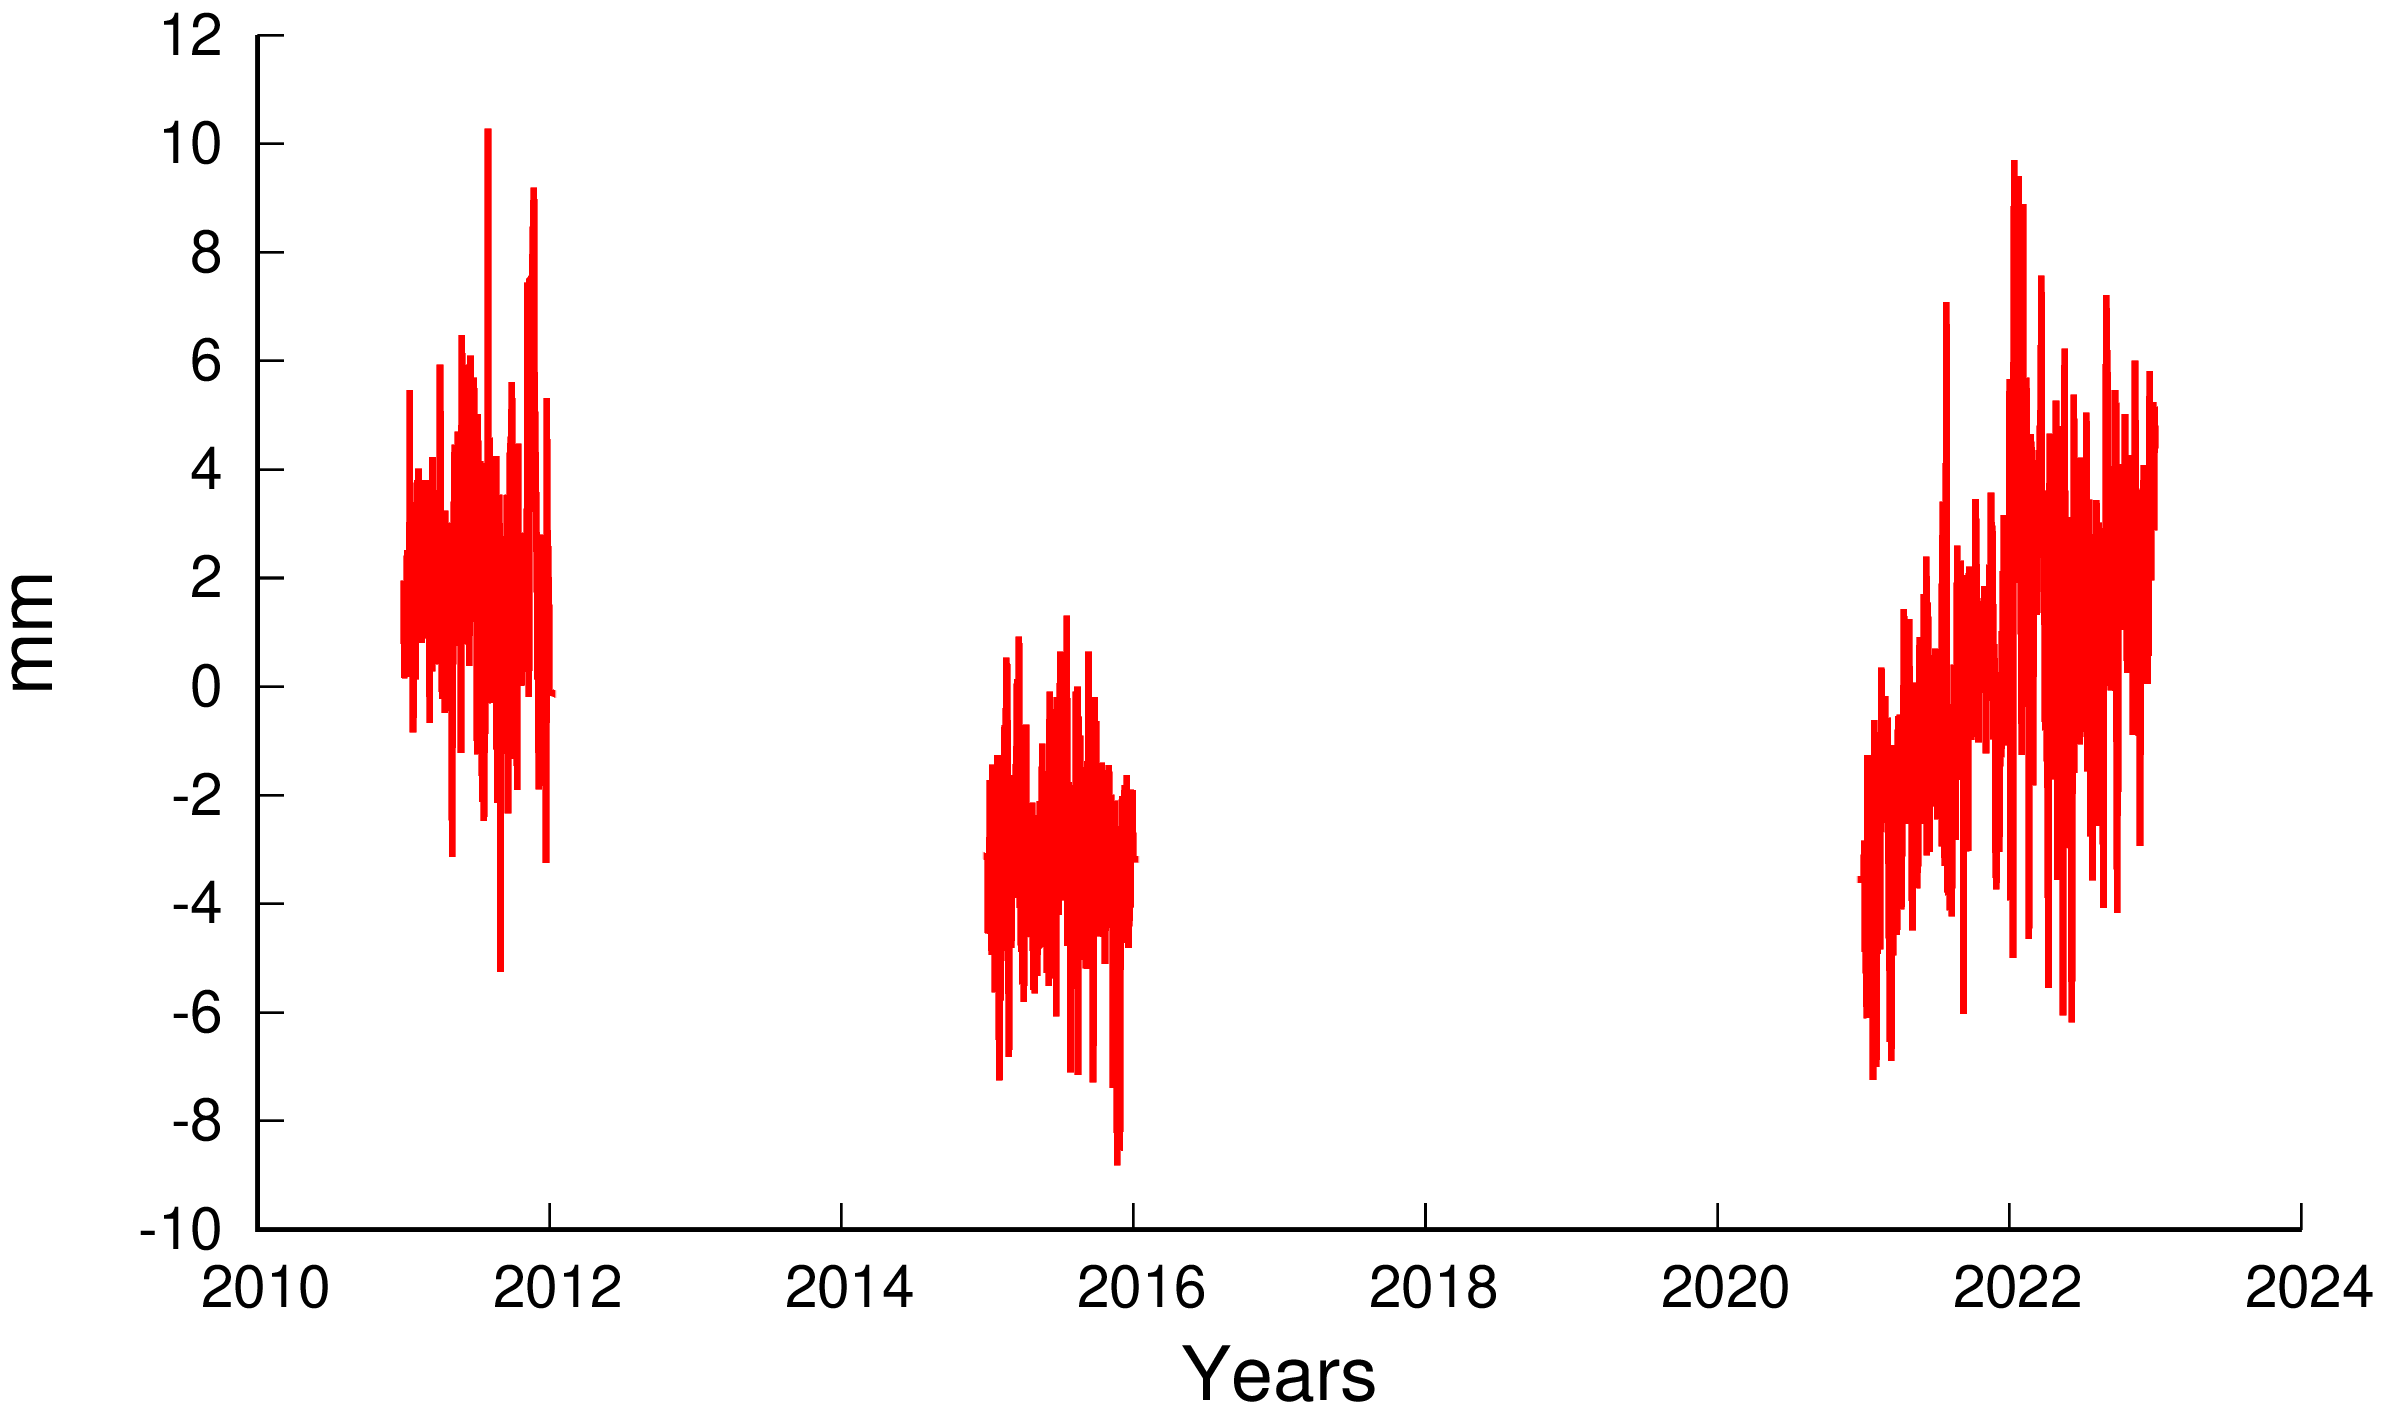
\includegraphics[height=5em]{057a_0_res.png}\\
%  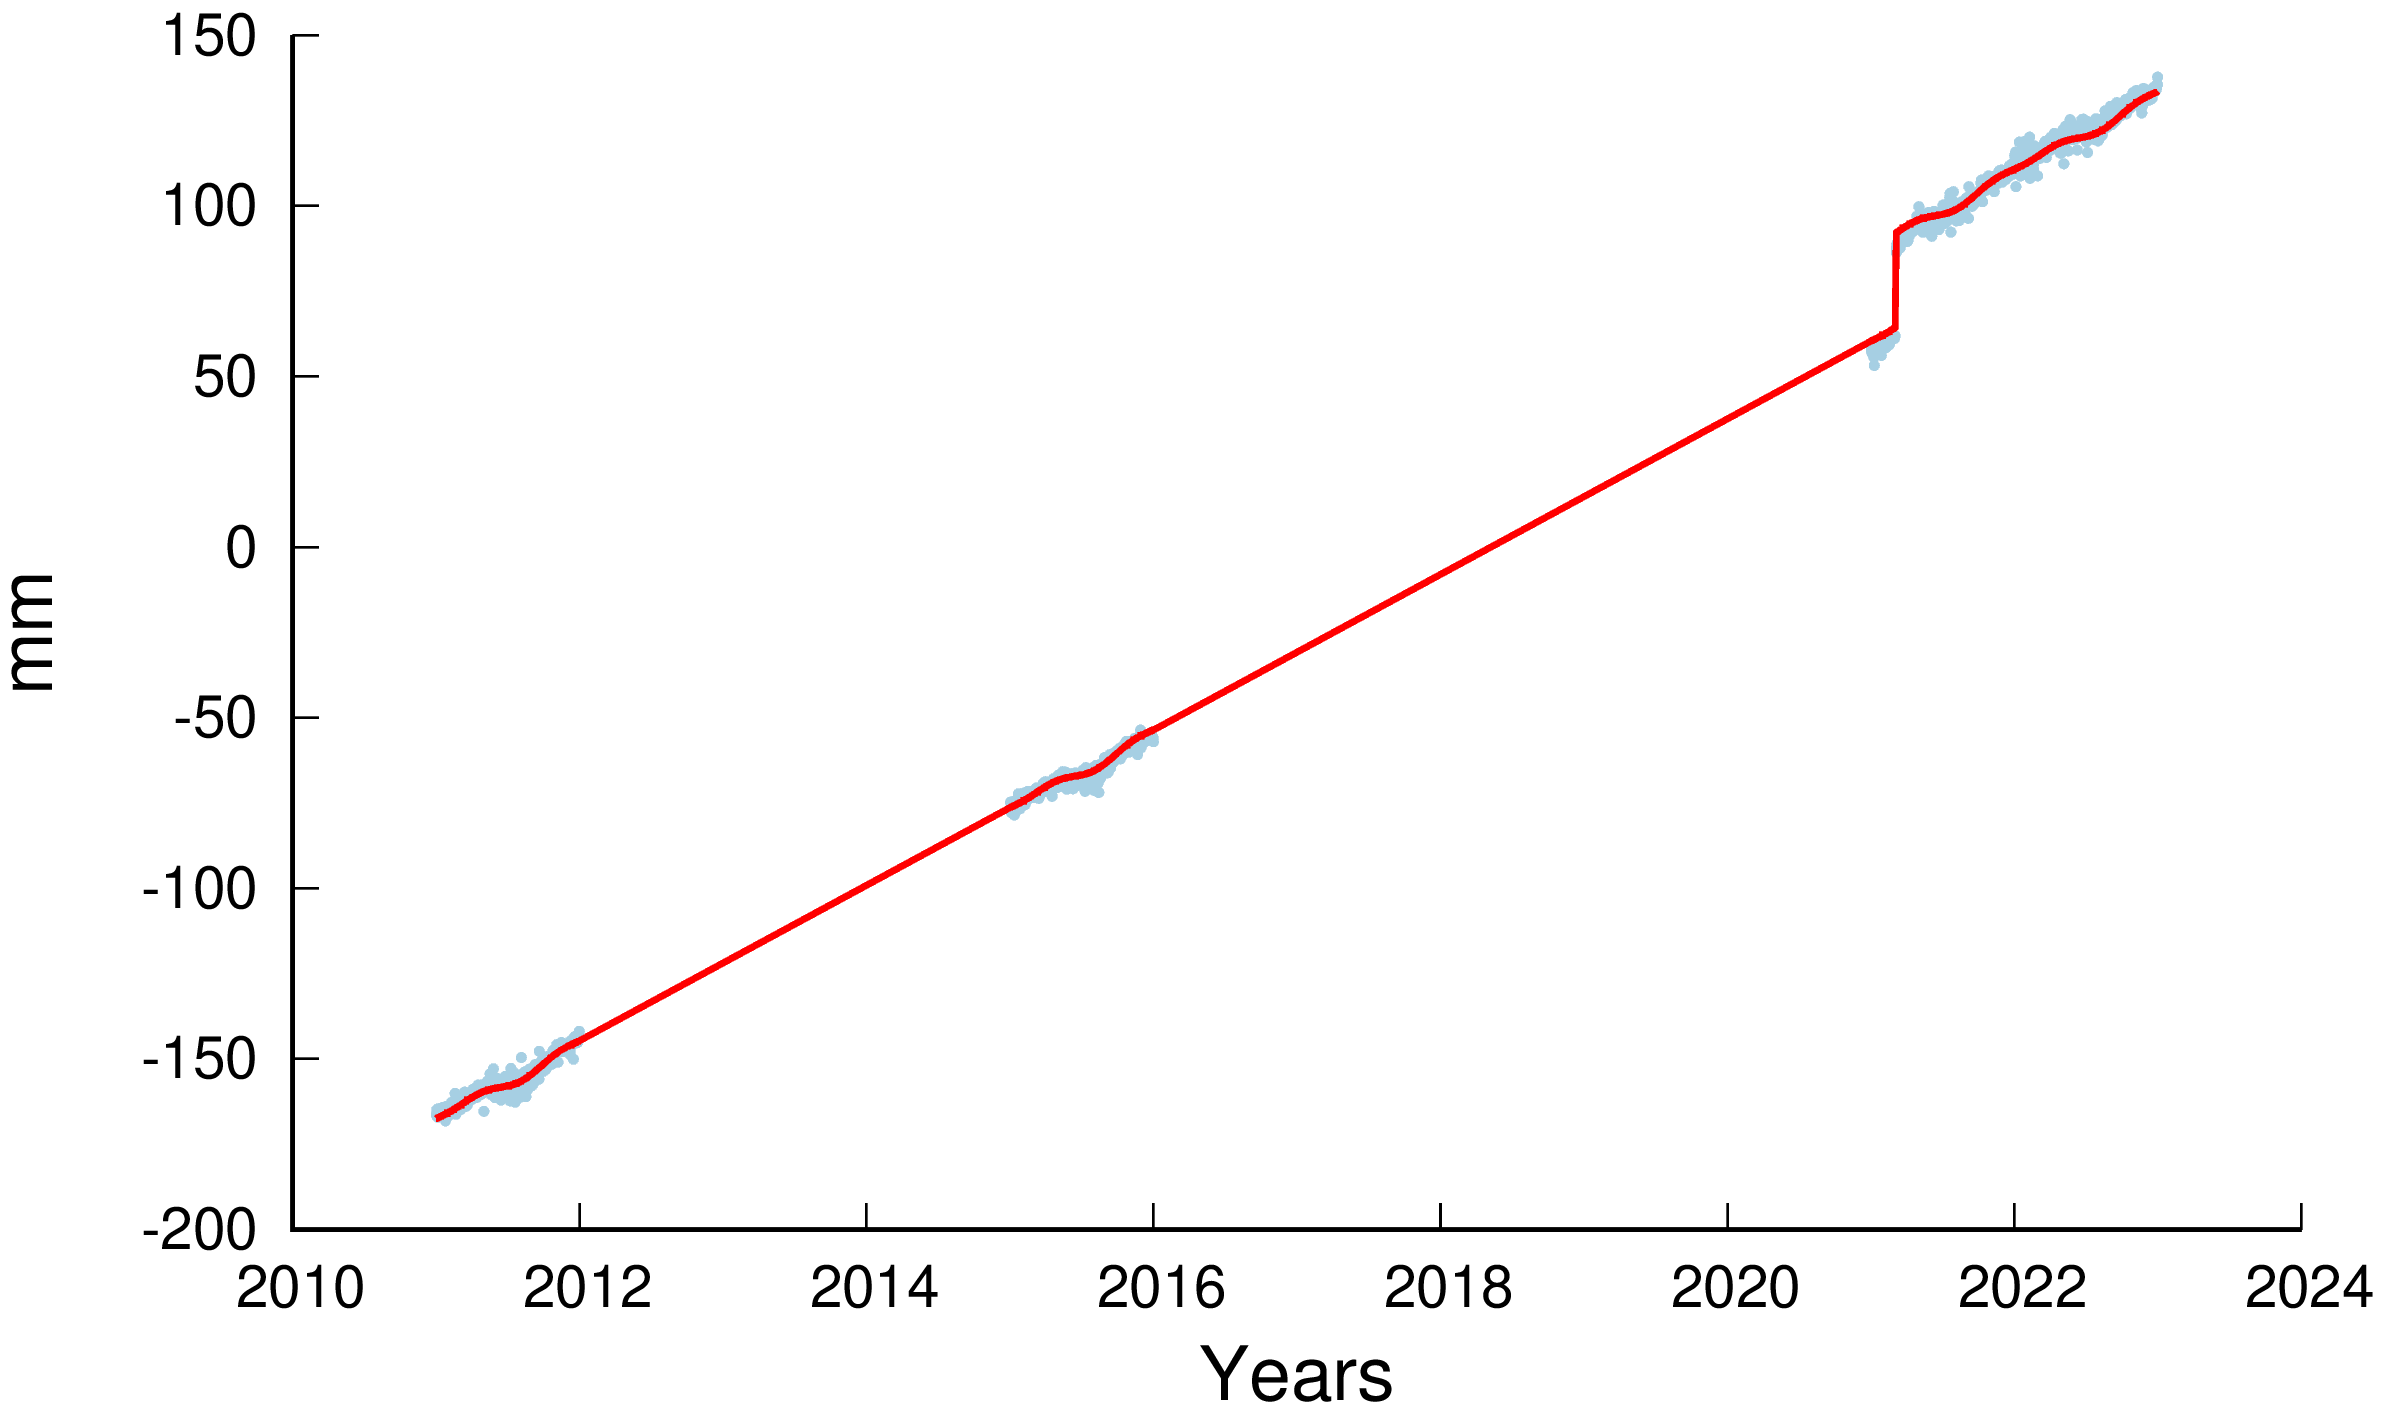
\includegraphics[height=5em]{057a_1_data.png}~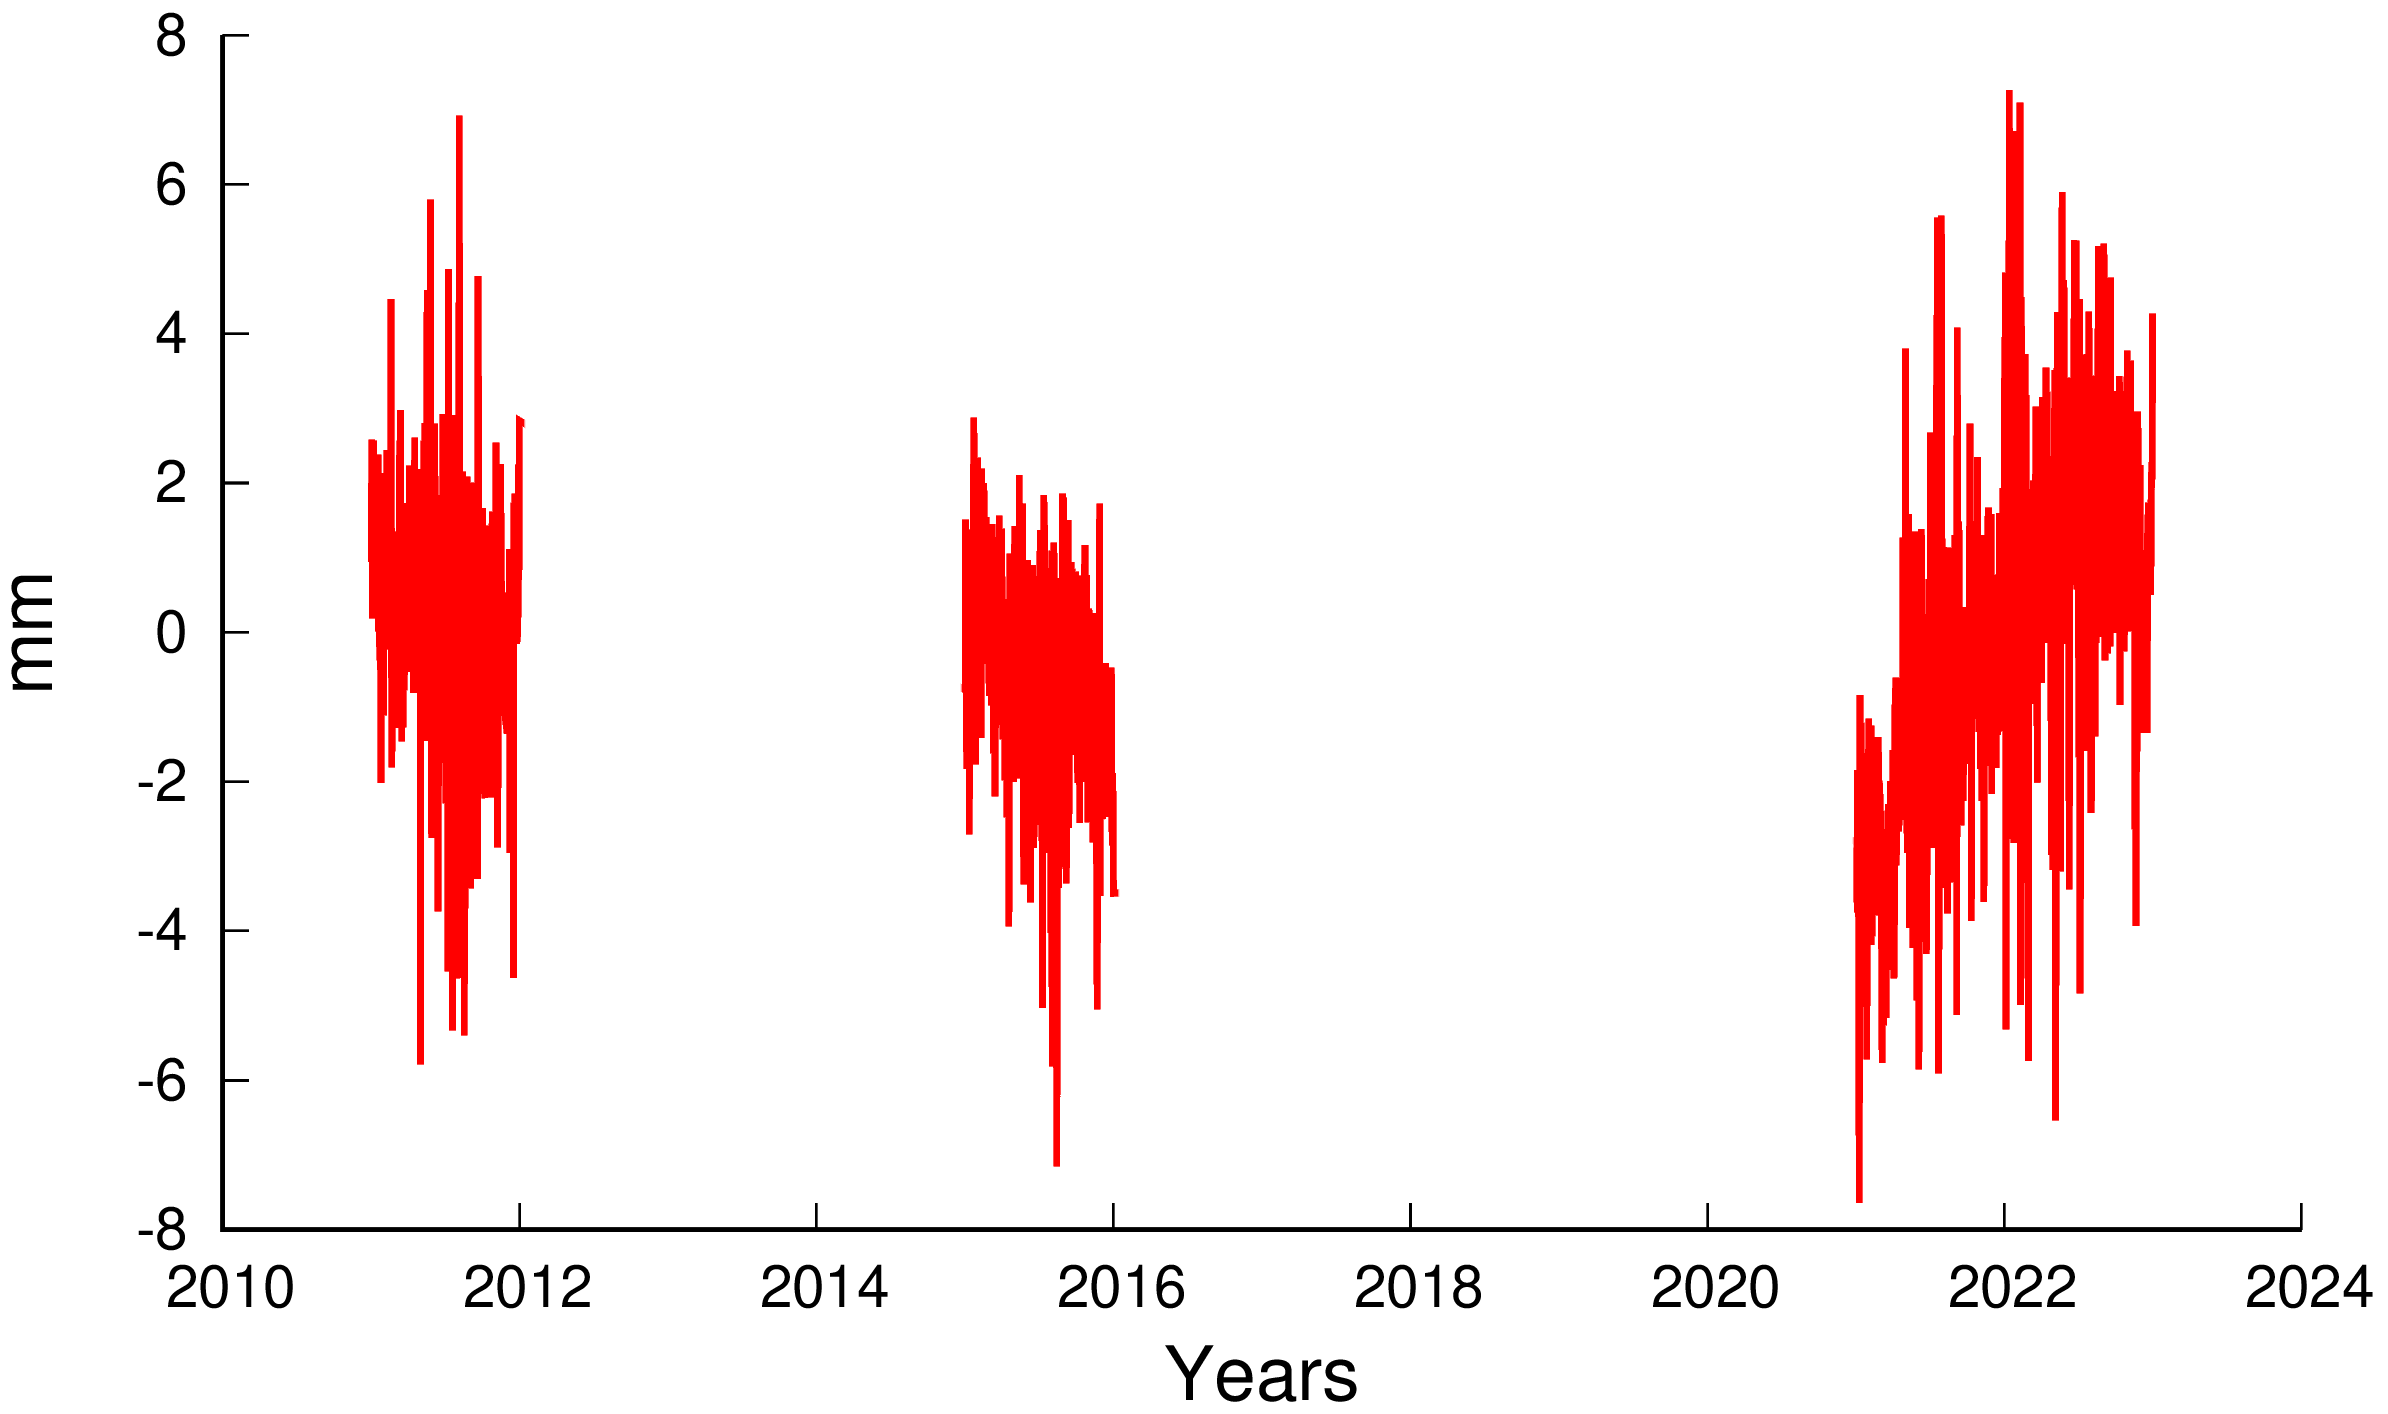
\includegraphics[height=5em]{057a_1_res.png}\\
%  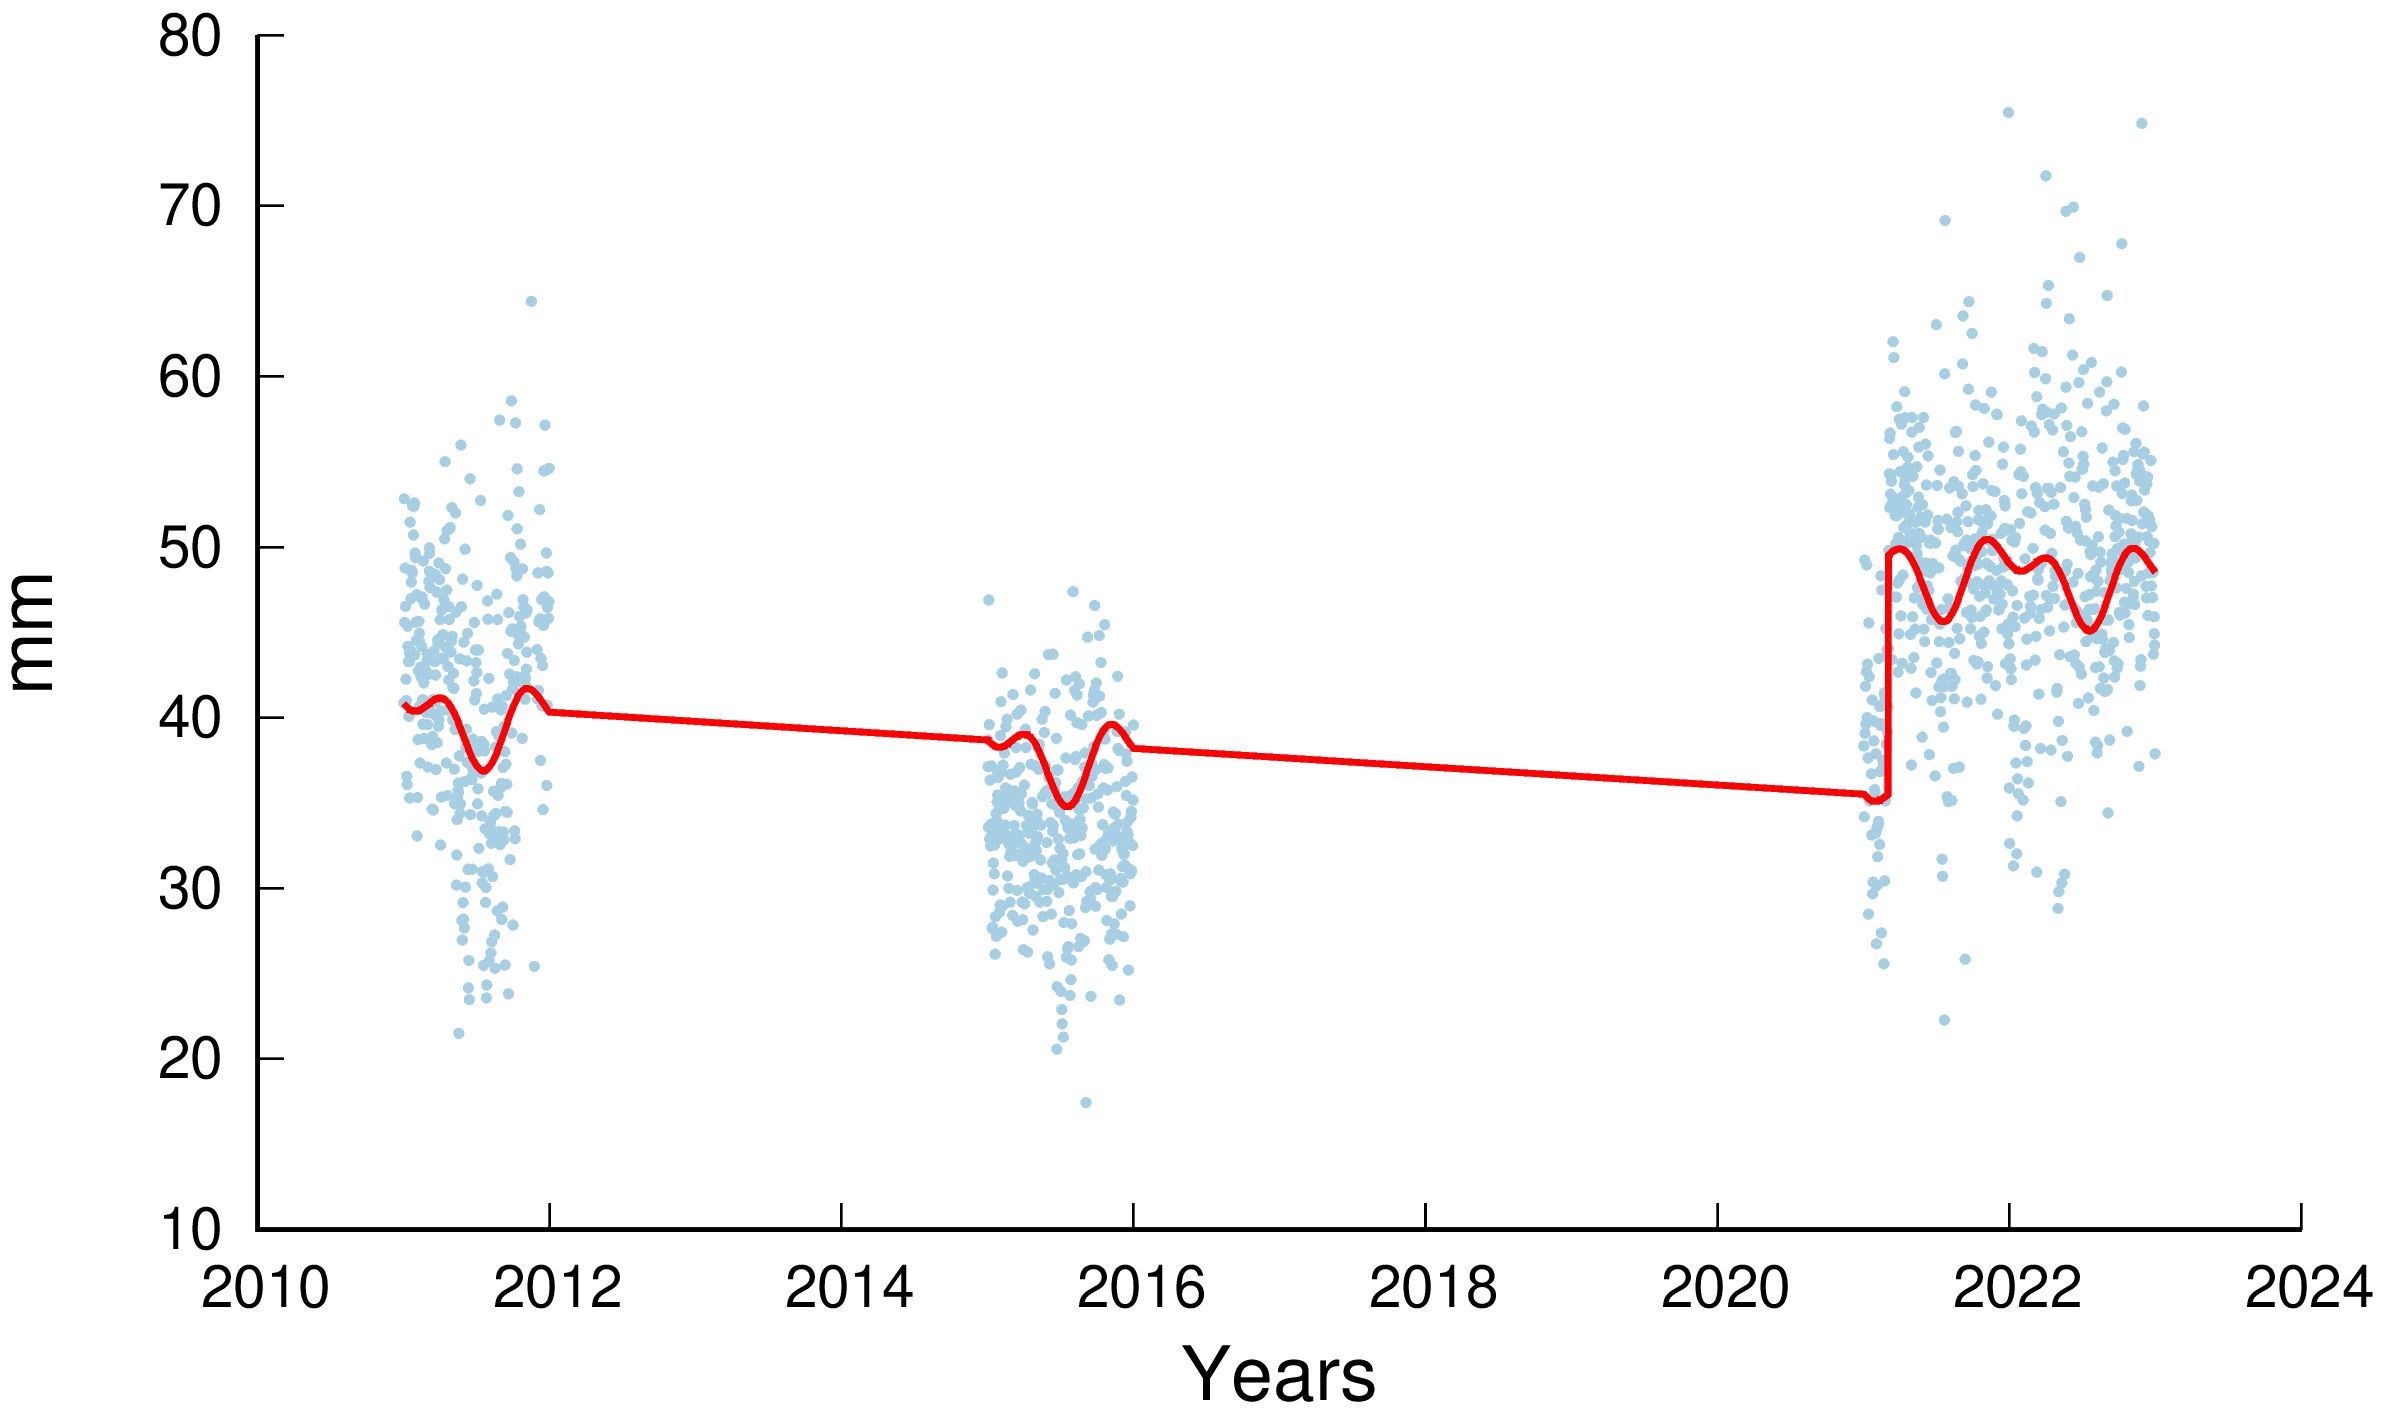
\includegraphics[height=5em]{057a_2_data.png}~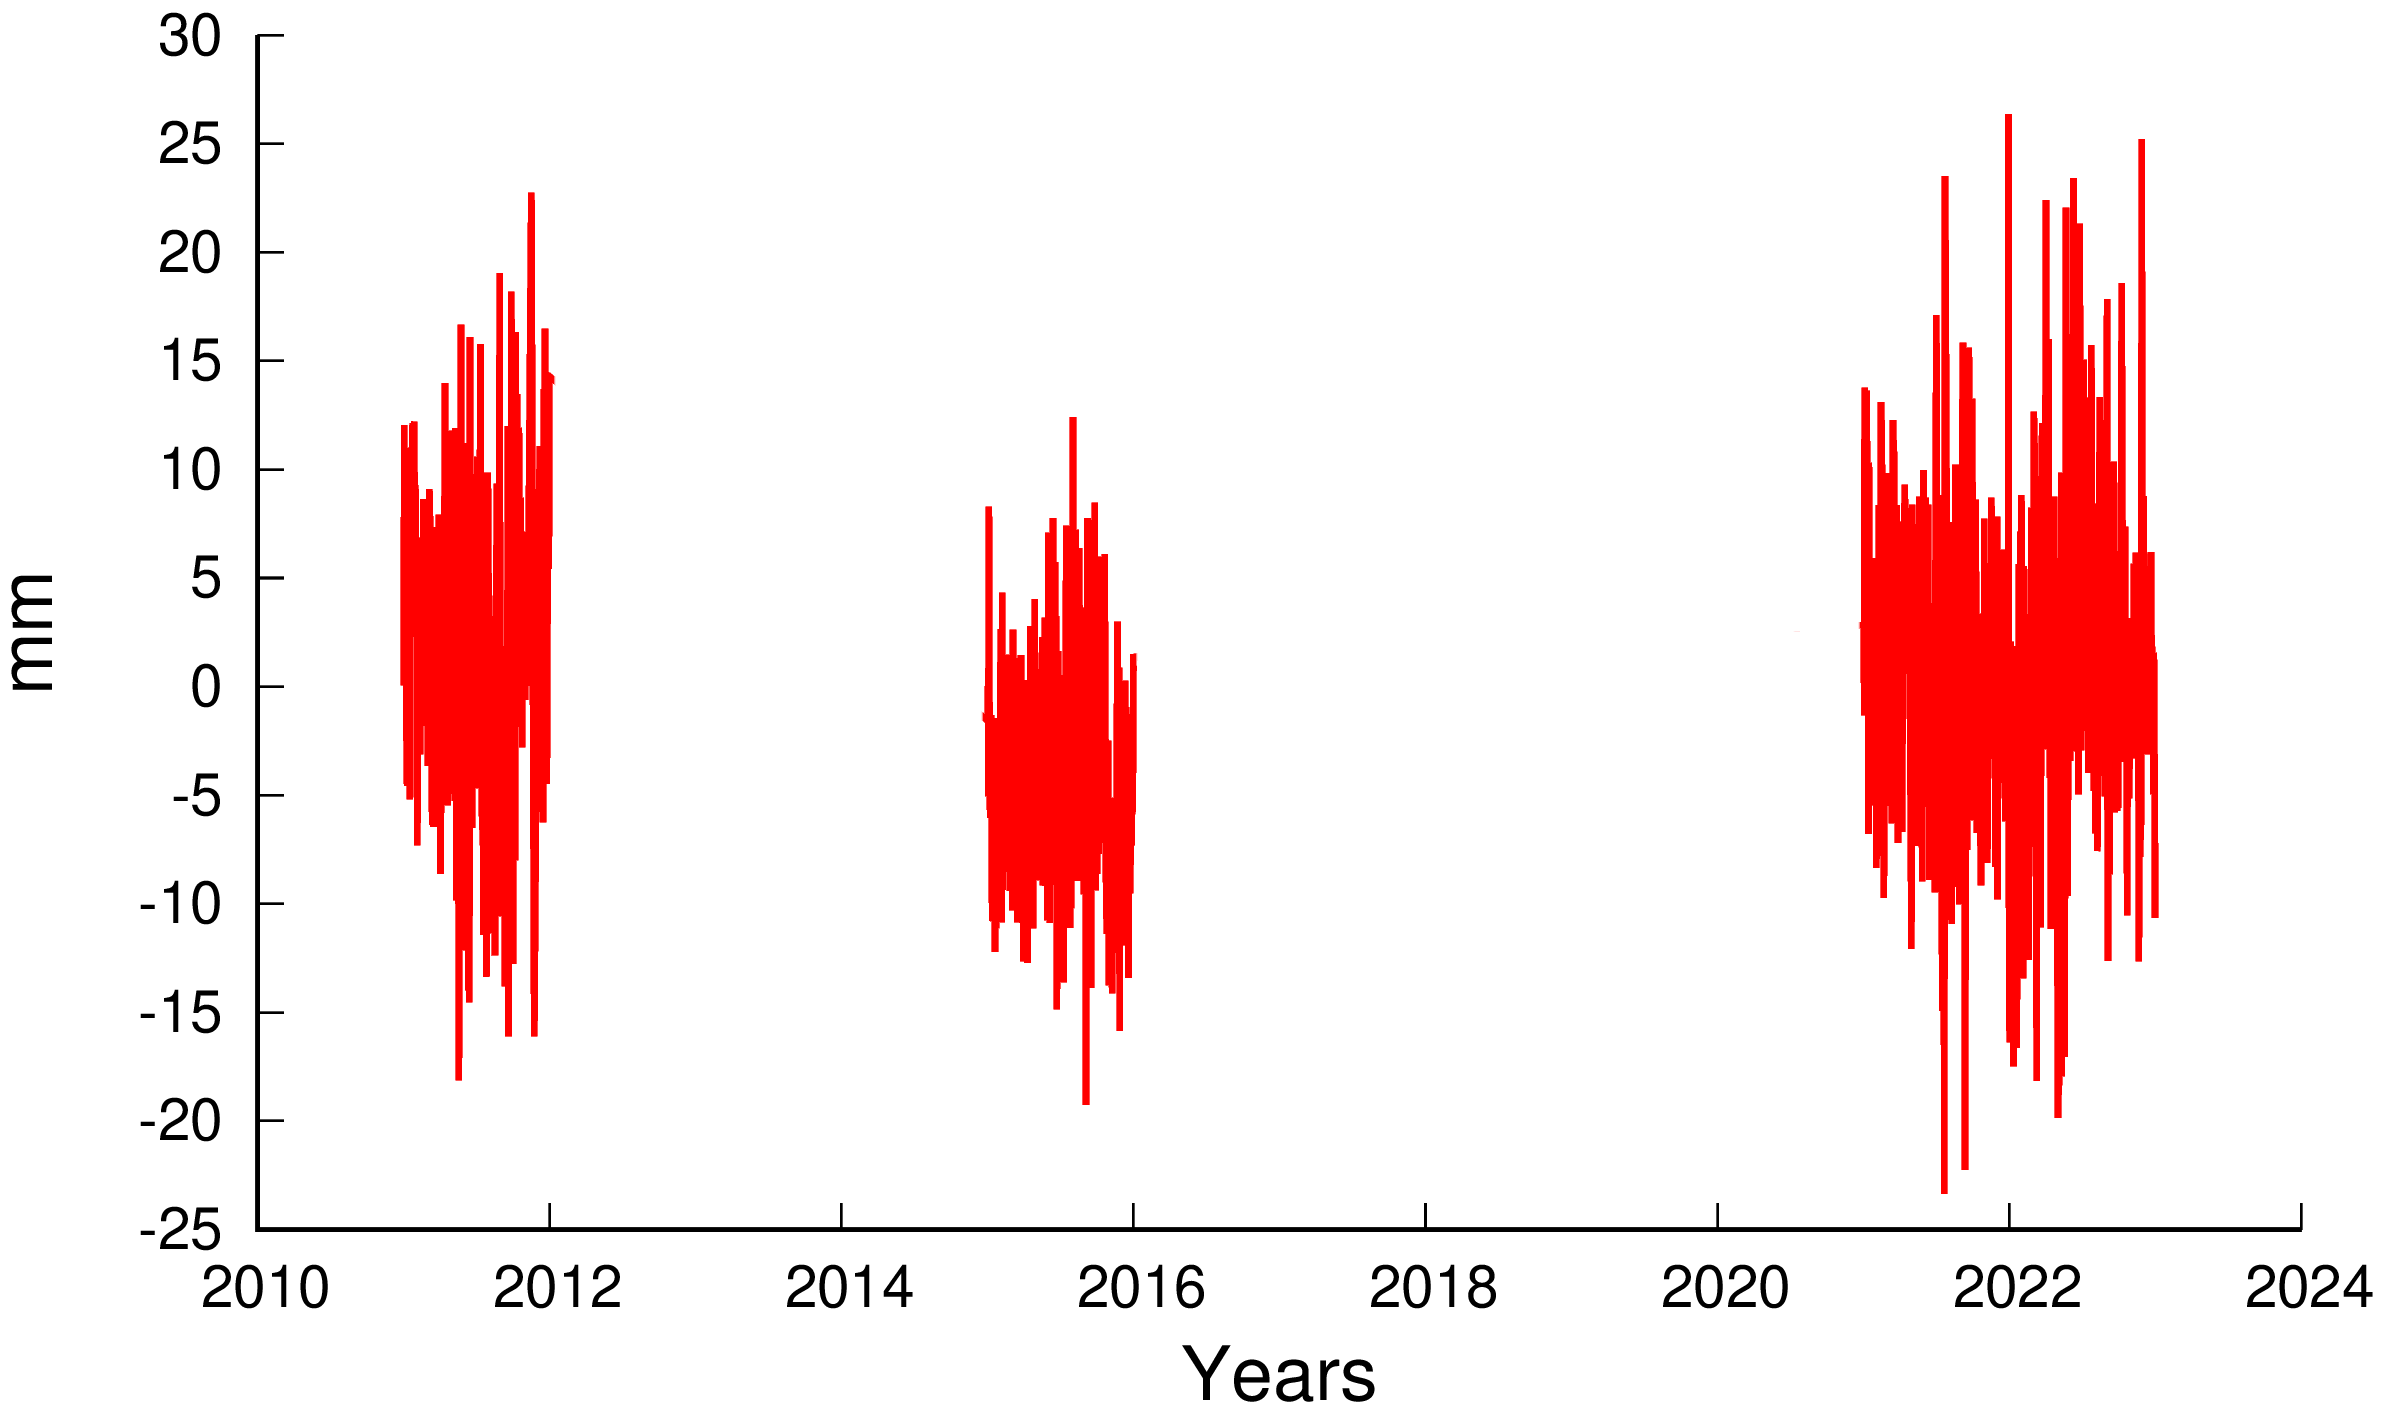
\includegraphics[height=5em]{057a_2_res.png}
%\end{minipage}
%\begin{minipage}[c]{0.33\linewidth}
%\begin{center}
%  040A (Santorini volcano inflation)
%\end{center}
%  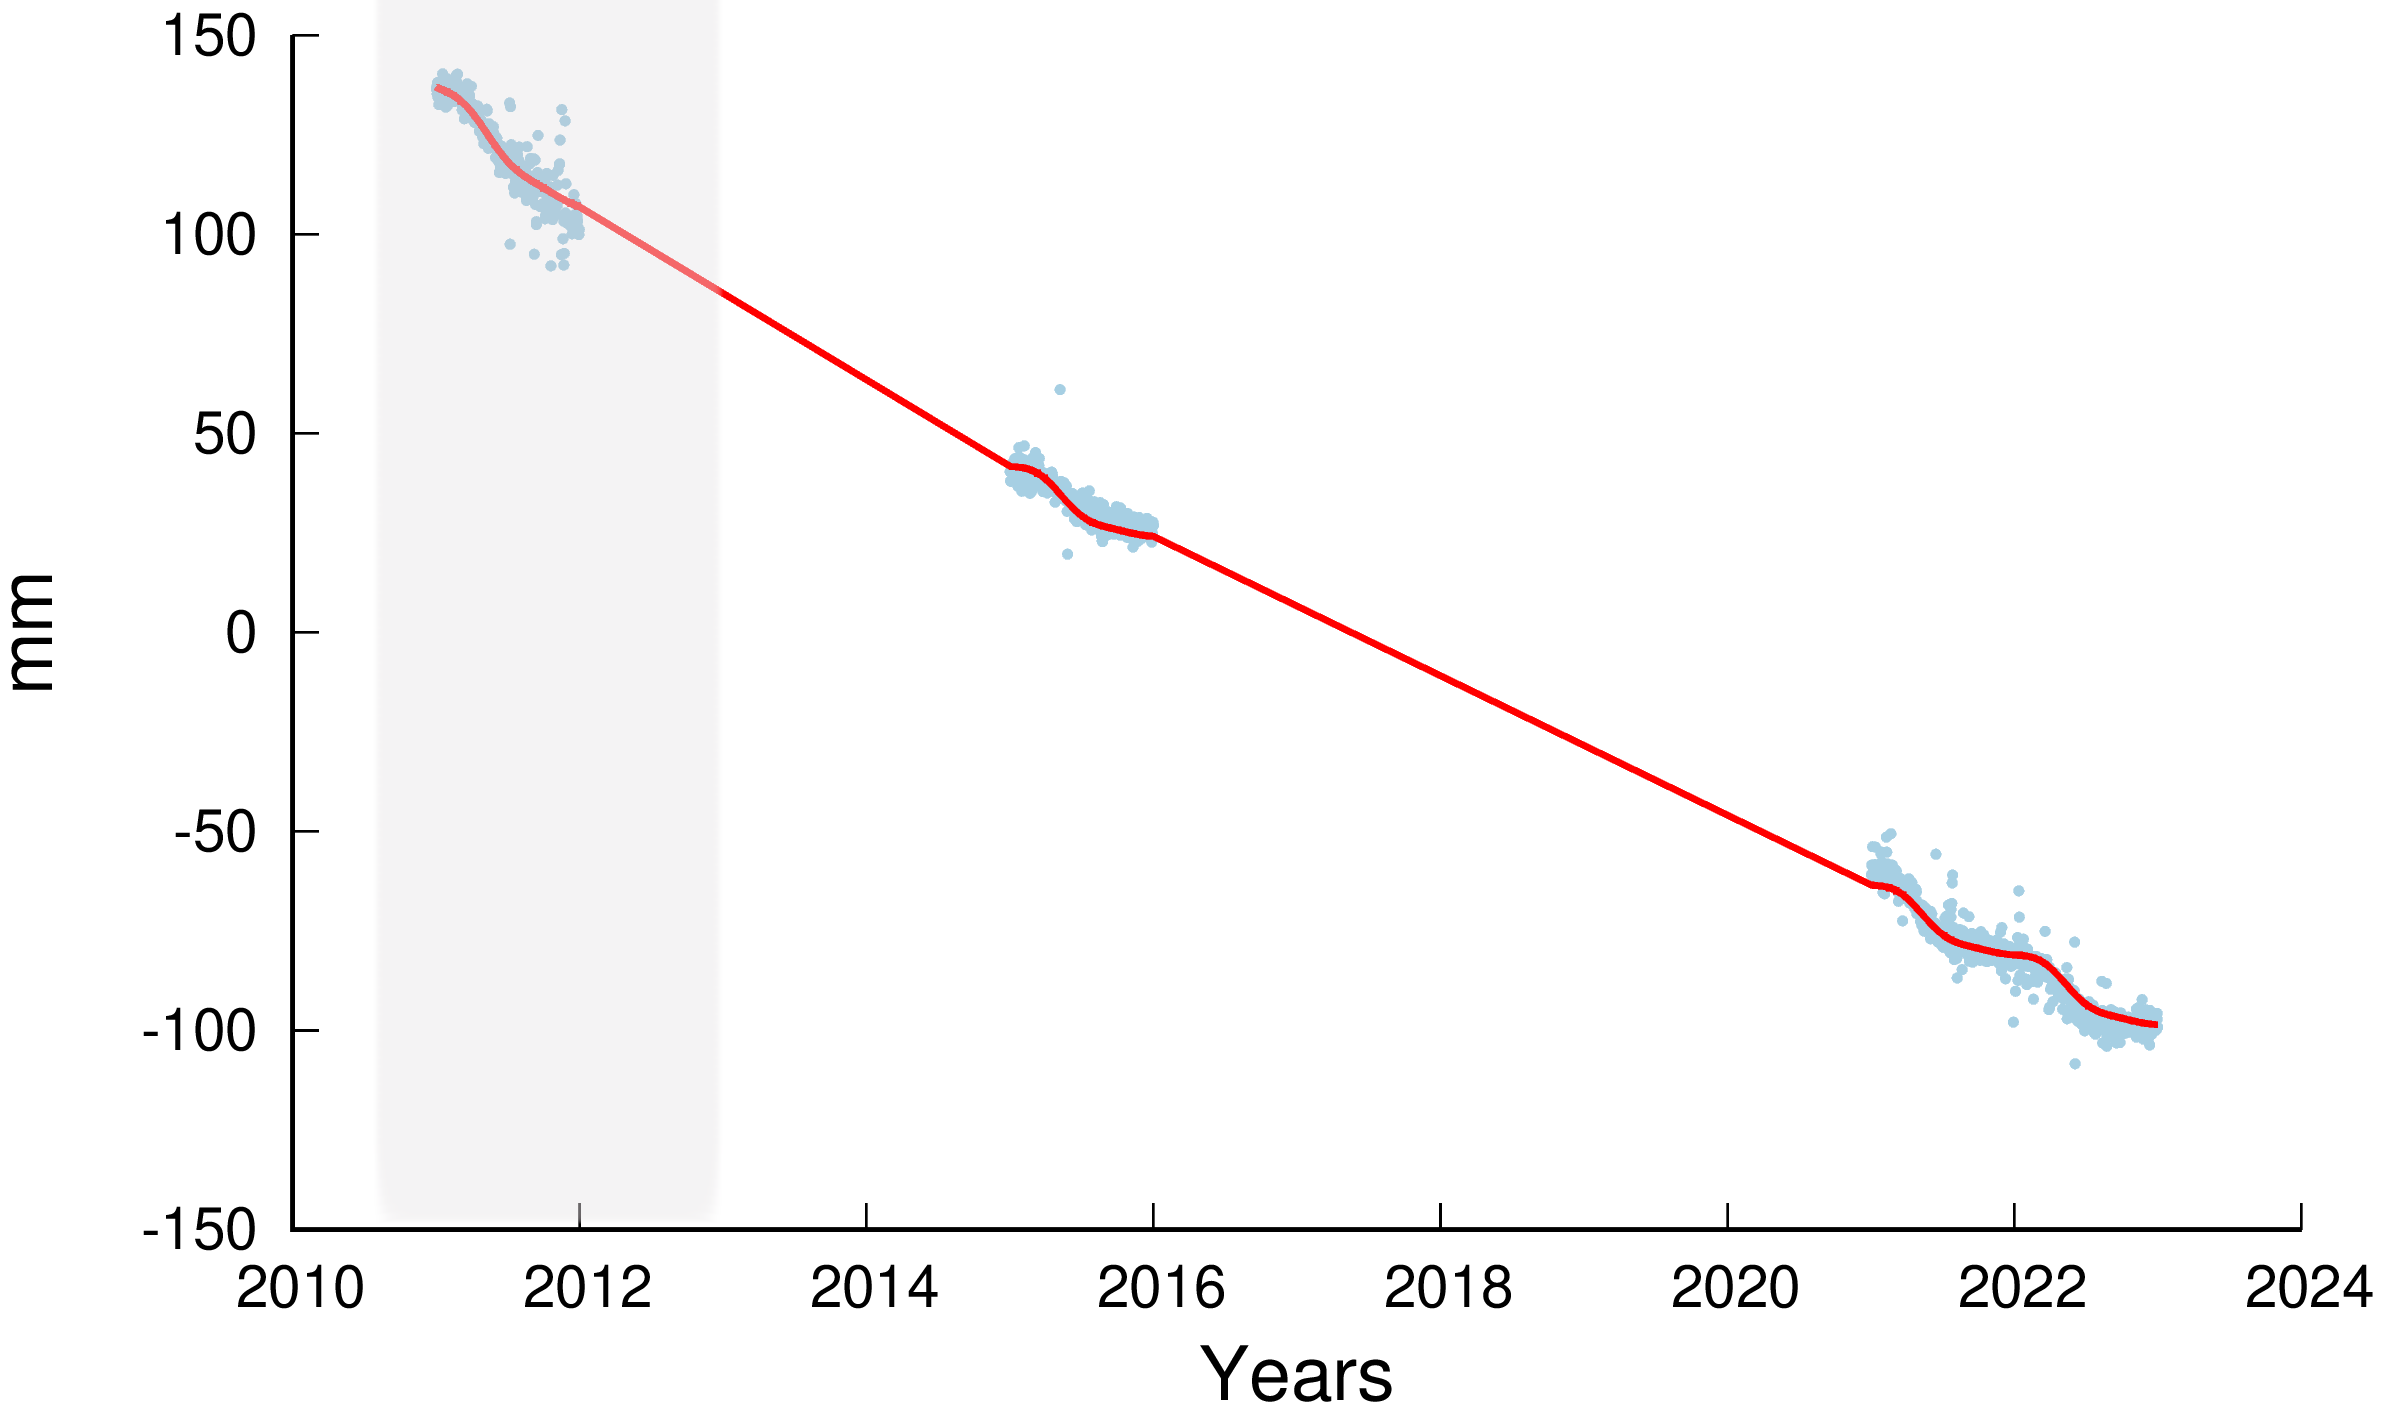
\includegraphics[height=5em]{048a_0_data.png}~
\includegraphics[height=5em]{048a_0_res.png}\\
%  
\includegraphics[height=5em]{048a_1_data.png}~
\includegraphics[height=5em]{048a_1_res.png}\\
%  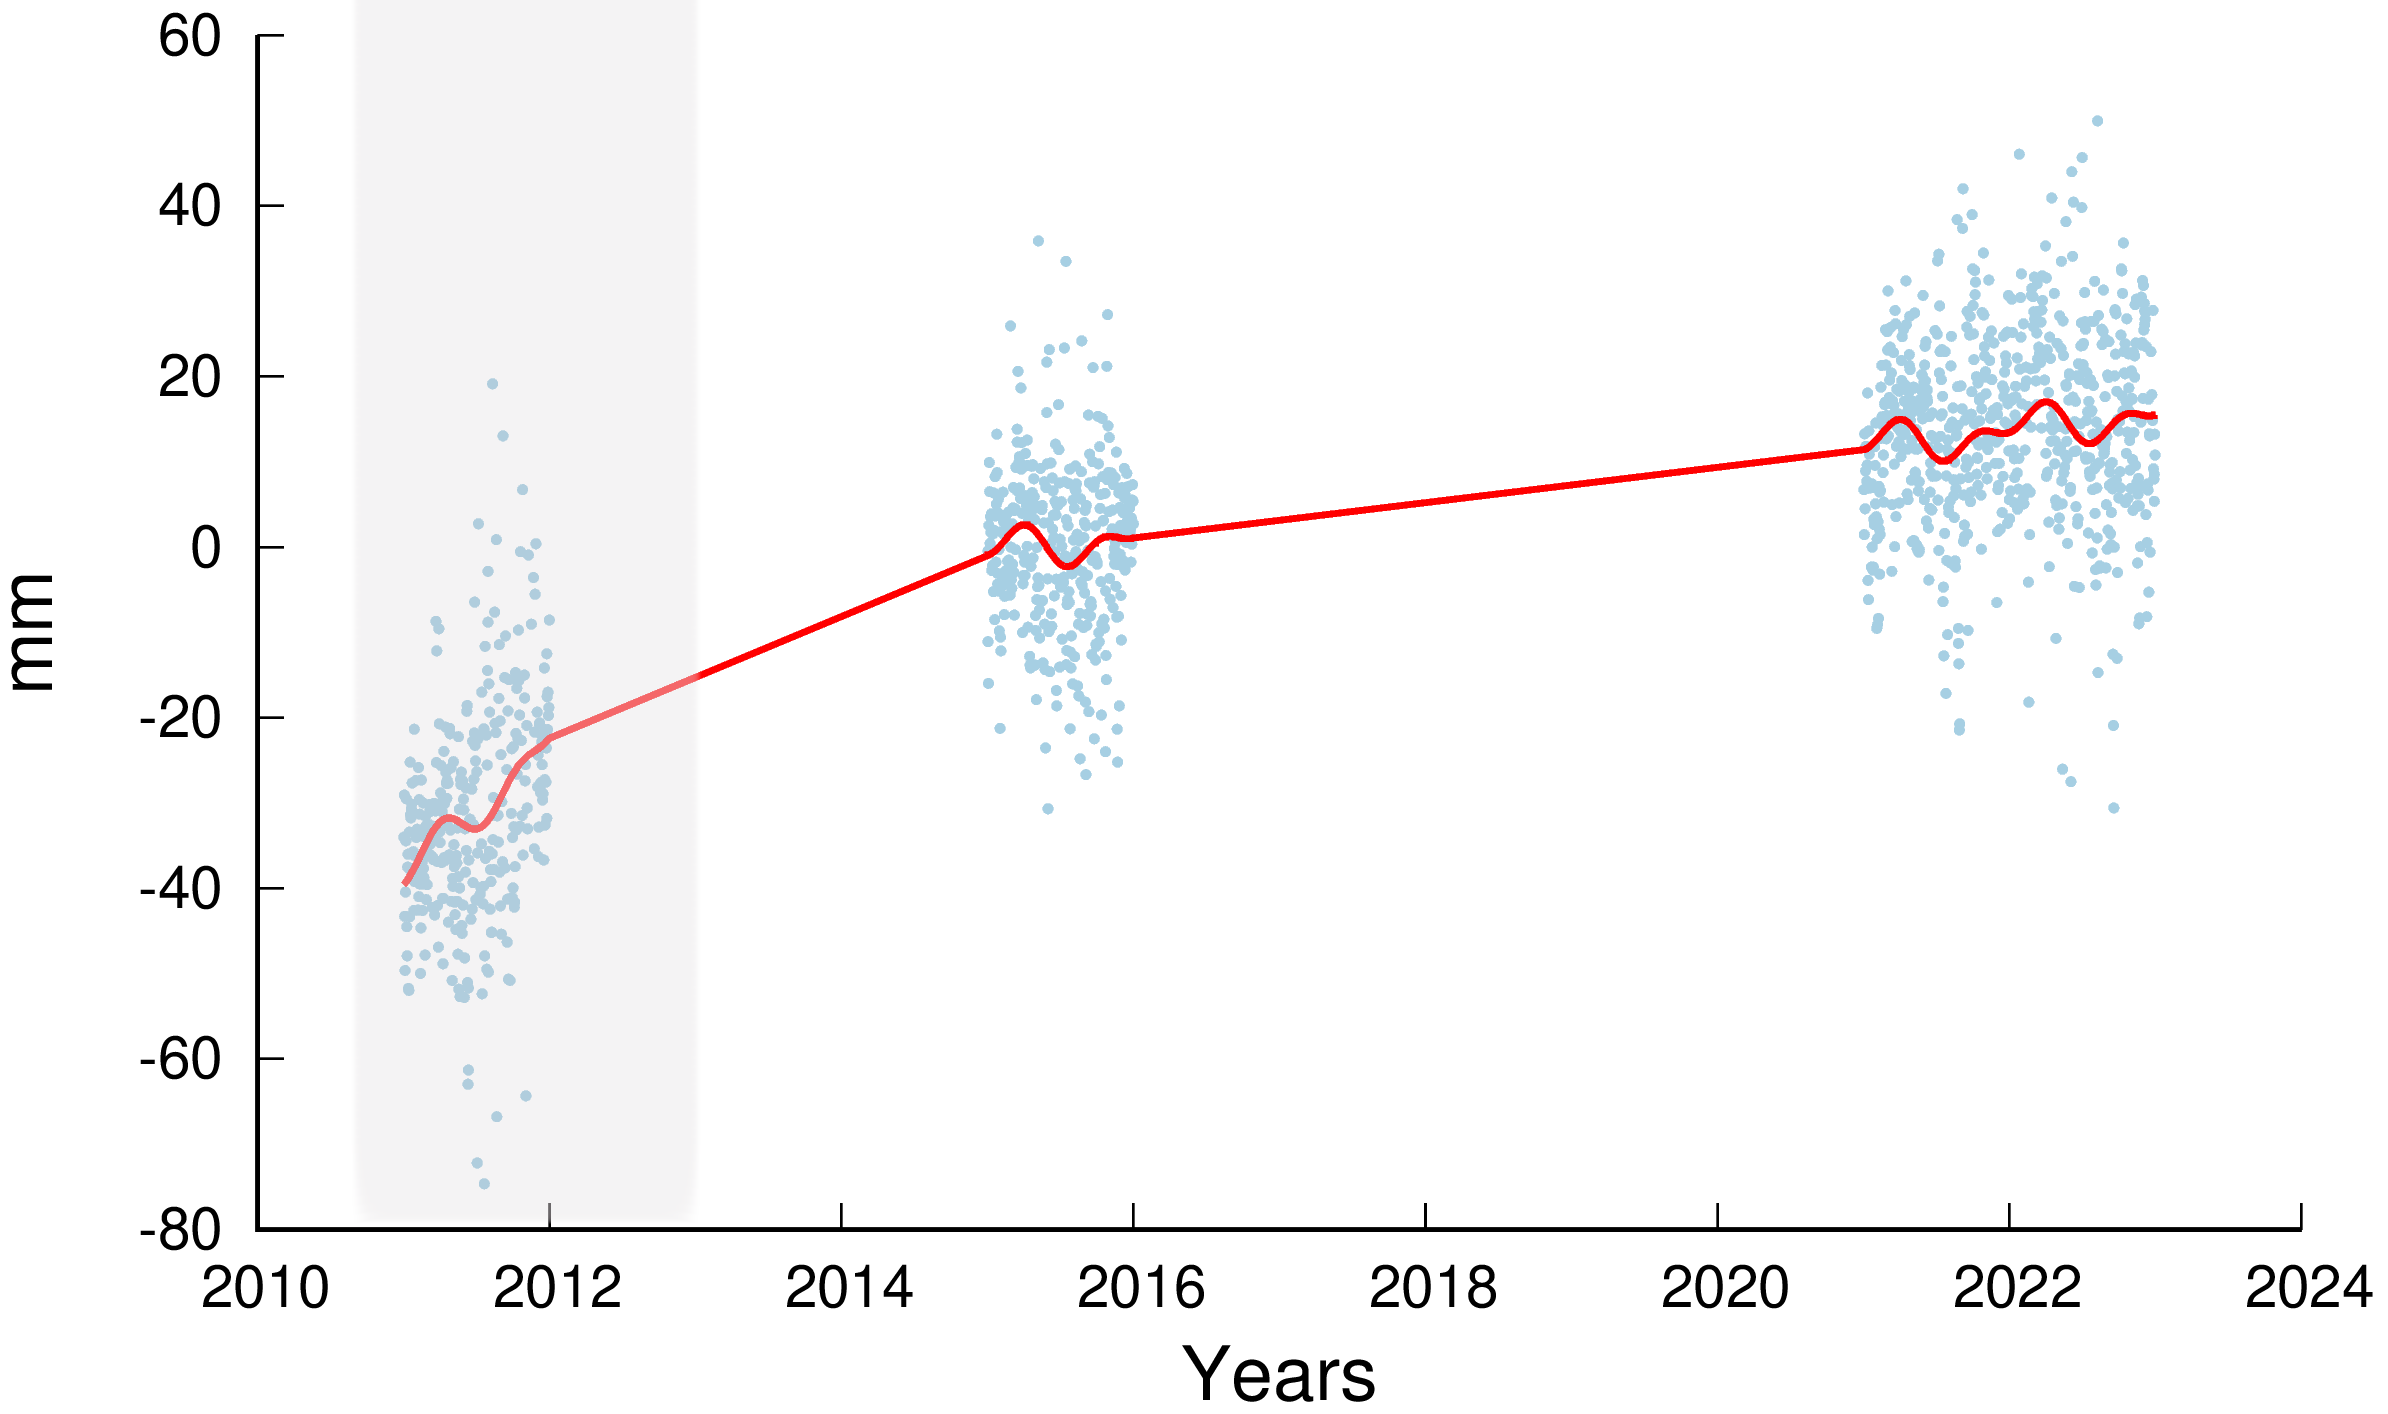
\includegraphics[height=5em]{048a_2_data.png}~
\includegraphics[height=5em]{048a_2_res.png}
%\end{minipage}

}

% %----------------------------------------------------------------------------------------
% %	RESULTS 1
% %----------------------------------------------------------------------------------------
% 
% \headerbox{Different Models Setup}{name=results,column=3,span=1,row=0}{
% 
% 
% }

%----------------------------------------------------------------------------------------
%	REFERENCES
%----------------------------------------------------------------------------------------
\renewcommand{\refname}{}
\let\oldthebibliography\thebibliography
\renewcommand{\thebibliography}[1]{%
  \oldthebibliography{#1}%
  \setlength{\itemsep}{0.2ex} % Less space between refs
  \setlength{\baselineskip}{0.9\baselineskip} % Optional line spacing tweak
}

\headerbox{References}{name=references,column=0, span=2, above=bottom}{
\label{refs}
\vspace*{-.3cm}
\begin{minipage}[b]{0.92\linewidth}
{\scriptsize
%\vspace*{-.4cm}
\nocite{*} % Insert publications even if they are not cited in the poster
\scriptsize{\bibliographystyle{unsrt}
\bibliography{sample}\vspace{0.01cm}} 
%\textbf{Anastasiou D.}, Papanikolaou P., Ganas A., and Paradissis D. (2021). “StrainTool: A software package to estimate strain tensor parameters (v1.0-r1)”. In: Zenodo. DOi:10.5281/zenodo.1297565. URL: https://doi.org/10.5281/zenodo.1297565
%
%\textbf{Bos, M. S.}, Fernandes, R. M. S., Williams, S. D. P., and Bastos, L. (2013). Fast Error Analysis of Continuous GNSS Observations with Missing Data.J. Geod., Vol. 87(4), 351–360, doi:10.1007/s00190-012-0605-0.
%
%\textbf{Dach, R.}, Lutz, P. Walser, P. Fridez (Eds); 2015: Bernese GNSS Software Version 5.2. User manual, Astronomical Institute, University of Bern, Bern Open Publishing. DOI: 10.7892/boris.72297; ISBN: 978-3-906813-05-9.
%
%\textbf{Wessel, P.}, W. H. F. Smith, R. Scharroo, J. F. Luis, and F. Wobbe, Generic Mapping Tools: Improved version released, EOS Trans. AGU, 94, 409-410, 2013
}
\end{minipage}
\begin{minipage}{0.06\linewidth}
%------------------------------------------
% \begin{wrapfigure}{c}{1.5cm}
\vspace*{-2.6cm}

\includegraphics[height=6em]{../../logos/graphic_egu_photo_yes.png}
% \caption{A wrapped figure going nicely inside the text.}\label{wrap-fig:1}
% \end{wrapfigure}
%------------------------------------------
\end{minipage}
}

%----------------------------------------------------------------------------------------
%	FUTURE RESEARCH
%----------------------------------------------------------------------------------------

\headerbox{Future Research}{name=futureresearch,column=2,aligned=references,above=bottom}{ 
\label{future_research}
{\footnotesize
%We consider this study to be a work-in-progress; we plan to go on with data analysis for all the available years. Currently, we are working on :
\begin{itemize}
\setlength\itemindent{0pt}
\setlength\leftskip{-16pt}
\setlength\itemsep{.01em}
  \item Investigate the co-seismic displacements of  the near-field GNSS stations.
  \item Investigate the far field of the directivity effect of the propagation seismic waves through the PGD of the GNSS stations.
  \item Investigate the frequency context of the seismic waves and its potential variation with the distance from the epicentre.
  \item Estimate of the seismic waves velocity as detected through the network GNSS stations displacement.
\end{itemize}
}
}

%----------------------------------------------------------------------------------------
%	FUNDING
%----------------------------------------------------------------------------------------

\headerbox{Contact Information}{name=funding,column=3,aligned=references,above=bottom}{ 
\label{Contact information}
\begin{minipage}[c]{.7\linewidth}
\begin{center}
\begin{tcolorbox}[height=2.5em,width=.97\textwidth,colback={airforceblue}, colupper=white,  boxrule=0pt]   
 \textbf{Abstract Number:  EGU2025-18416}
\end{tcolorbox}  
 \end{center}
 \vspace*{-.2cm}
 \textbf{Dimitrios Anastasiou}\\
 \textit{Assistant Professor NTUA}\\
 danastasiou@mail.ntua.gr
\end{minipage}
\begin{minipage}[c]{.27\linewidth}
\begin{center}
  
\includegraphics[width=.93\textwidth]{egu25-18416-qr.png}
\end{center}
\end{minipage}


}

%----------------------------------------------------------------------------------------
%	RESULTS 2
%----------------------------------------------------------------------------------------

\headerbox{Discussion}{name=resval,column=2,span=2,row=0,below=data,above=references}{
\label{discussion}

\begin{minipage}{0.603\textwidth}
\begin{minipage}{\textwidth}
  \begin{minipage}{0.48\textwidth}
    \begin{center}
    \textbf{Near-field}
      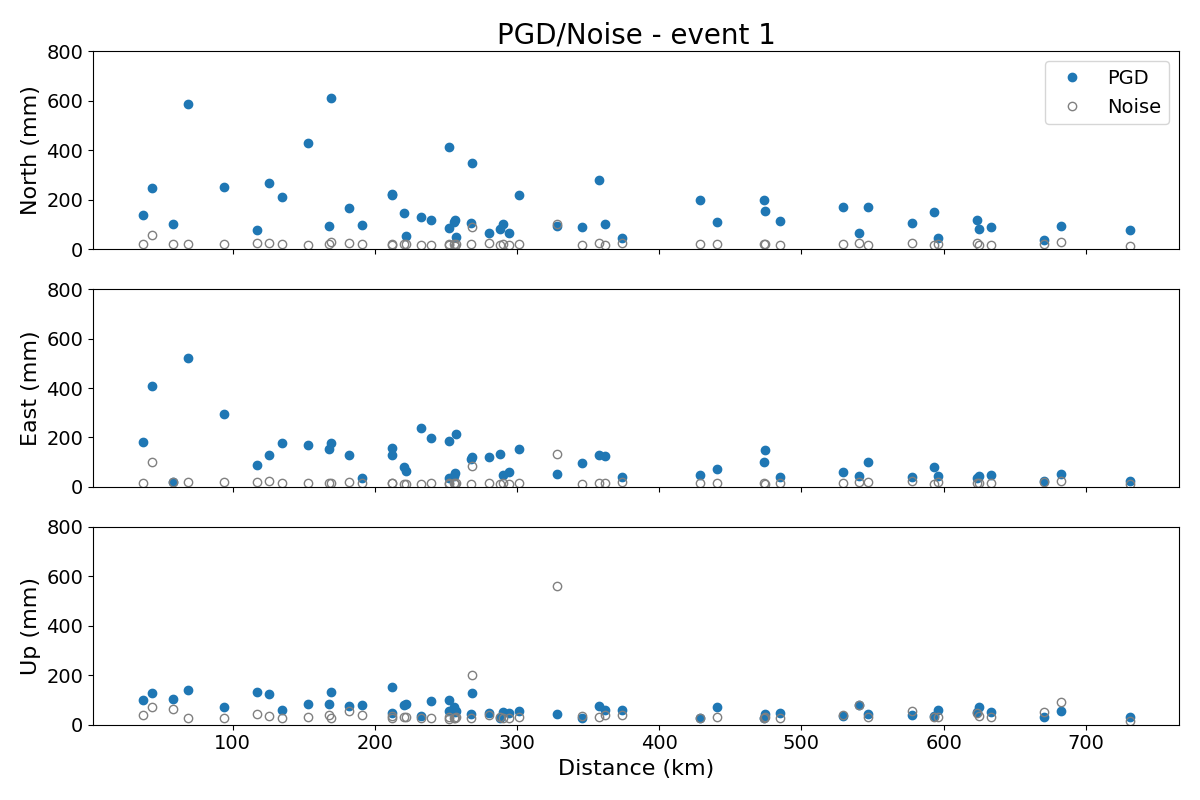
\includegraphics[width=.97\textwidth]{PGD_eq1tr.png}
    \end{center}
  \end{minipage}
  \begin{minipage}{0.48\textwidth}
    \begin{center}
    \textbf{Far-field}
      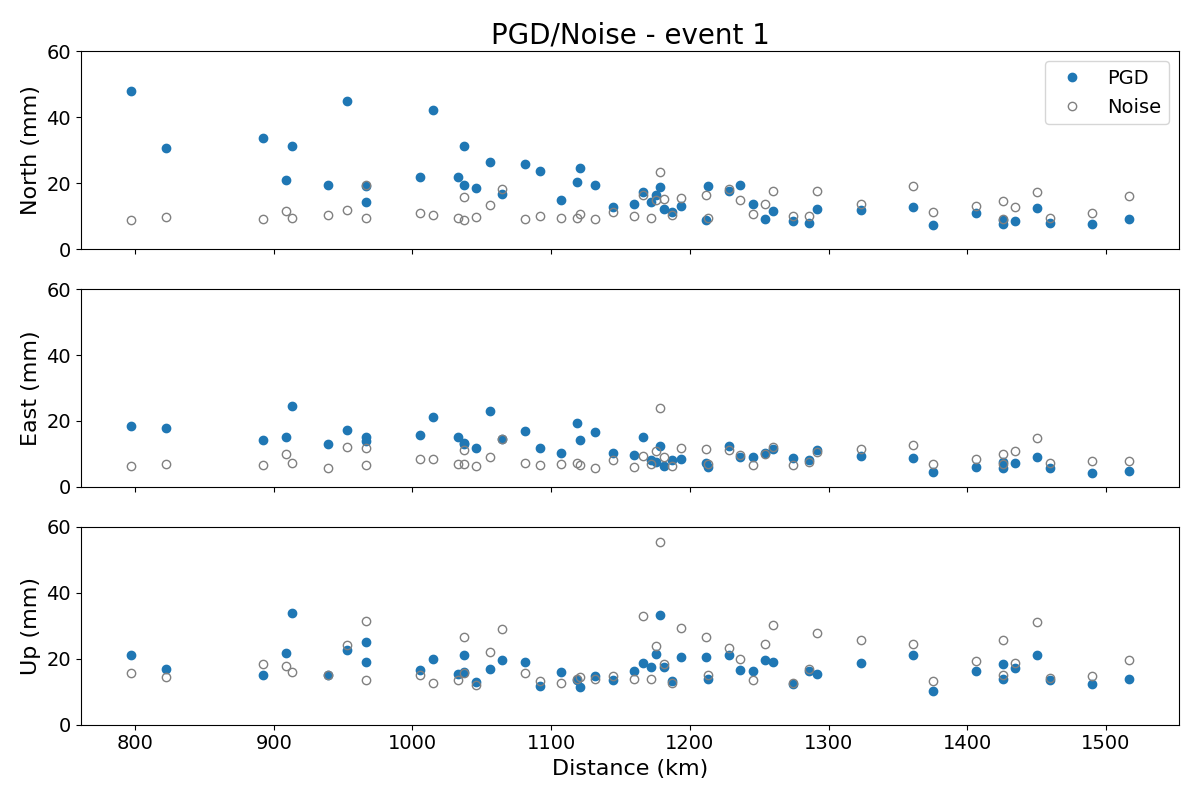
\includegraphics[width=.97\textwidth]{PGD_eq1gr.png}
    \end{center}
  \end{minipage}
\end{minipage}

\begin{minipage}{\textwidth}
  \begin{minipage}{0.48\textwidth}
    \begin{center}
      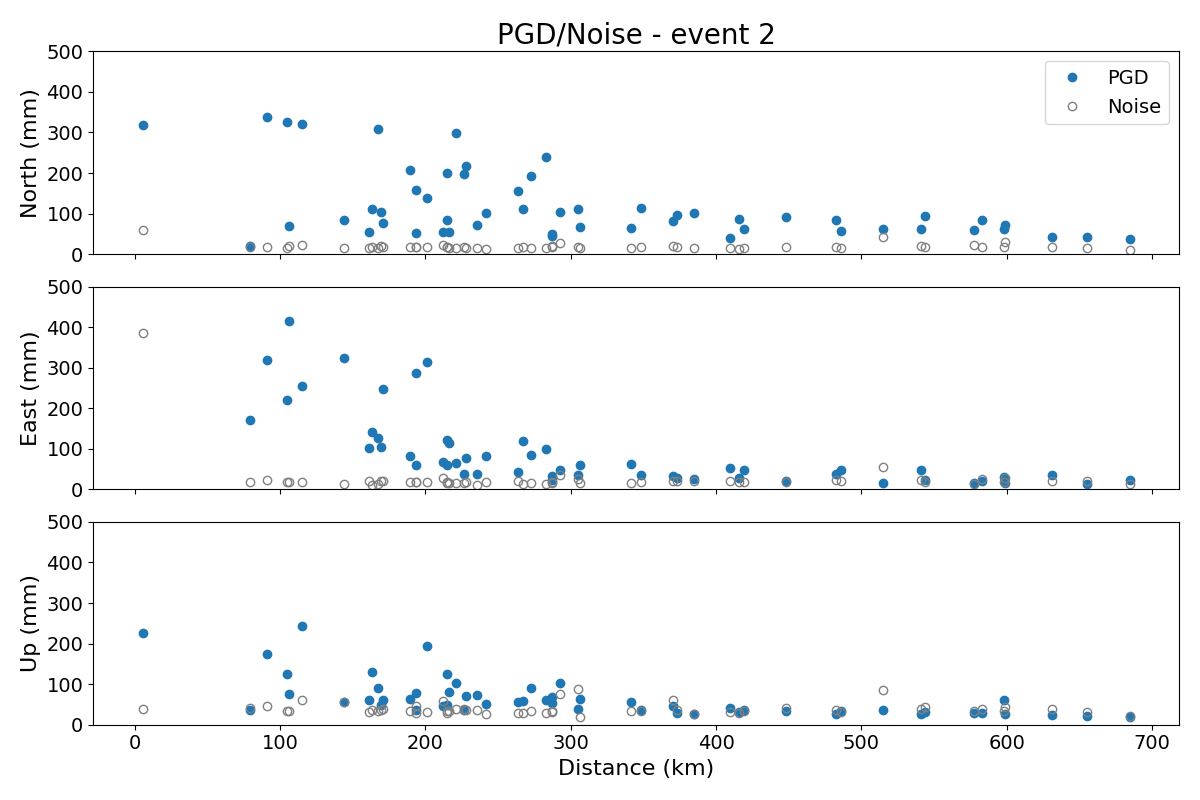
\includegraphics[width=.97\textwidth]{PGD_eq2tr.png}
    \end{center}
  \end{minipage}
  \begin{minipage}{0.48\textwidth}
    \begin{center}
      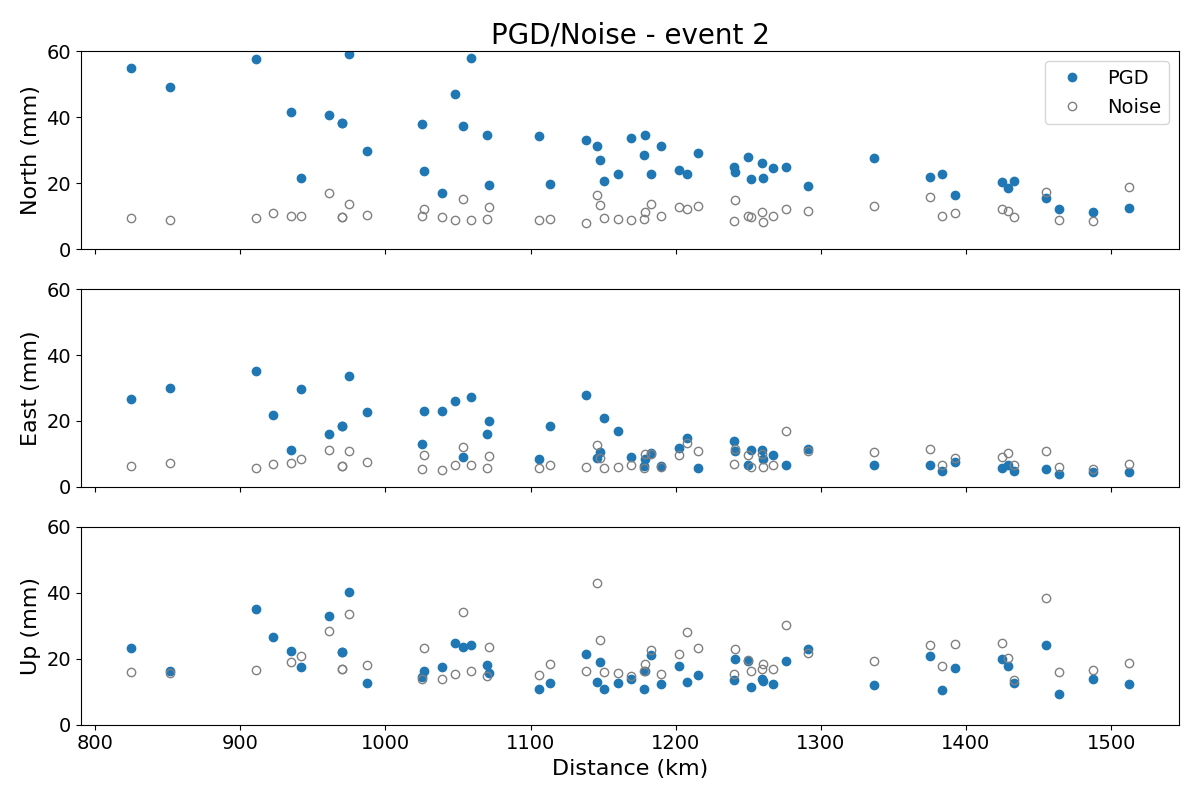
\includegraphics[width=.97\textwidth]{PGD_eq2gr.png}
    \end{center}
  \end{minipage}
 \end{minipage} 
\end{minipage}
\begin{minipage}{.395\textwidth}
Preliminary results from PGD values:\\[-.6cm]
\begin{itemize}
\setlength\itemindent{0pt}
\setlength\leftskip{-24pt}
\setlength\itemsep{.01em}
  \item The highest PGD values (up to 60 cm) are observed at near-field stations located within 300 km of the epicenters.
  \item PGD values generally decrease with distance from the epicenters. However, due to the directivity of seismic wave propagation and fault orientation.
  \item The highest PGD values are observed at the North component for both seismic events, indicating that the North-South direction is mostly affected by the propagation of the seismic waves.
  \item The second seismic event has a larger far-field impact, probably due to the geometry of the seismic fault and the directivity of the seismic waves propagation.
  \item The Up component is not affected by the seismic events potentially due to the small impact that the S-waves may have for far-field stations.
%  \item The PGD values tend to decrease with the distance from the epicetres. However it is obvious the impact of the directivity of the propagation of the seismic waves and the orientation of the seismic faults, as the PGD values of GNSS stations of similar distance from the epicentres has large range. For instance, the PGD values of the northing component of GNSS stations with ~1000km epicentre distance for the second seismic event range between 20 to 60cm.
\end{itemize}
\end{minipage}
\vskip.4cm
}

%----------------------------------------------------------------------------------------
%	HEPOS NETWORK
%----------------------------------------------------------------------------------------

\headerbox{GNSS stations}{name=heposnet,column=0,below=introduction,bottomaligned=resval}{ 
\label{datanet}
A network of 95 continuous GNSS stations was utilized for this study, comprising:
a) 41 continuously operating stations located near the earthquake sequence in
southwest Turkey (<700km distance from epicentre, red points) and b) 54 far-field stations
distributed across the Aegean Sea and mainland Greece, located 800 to 1600 km
from the epicentres of the two earthquakes (blue points). 

\begin{minipage}[c]{0.97\linewidth}
  \fbox{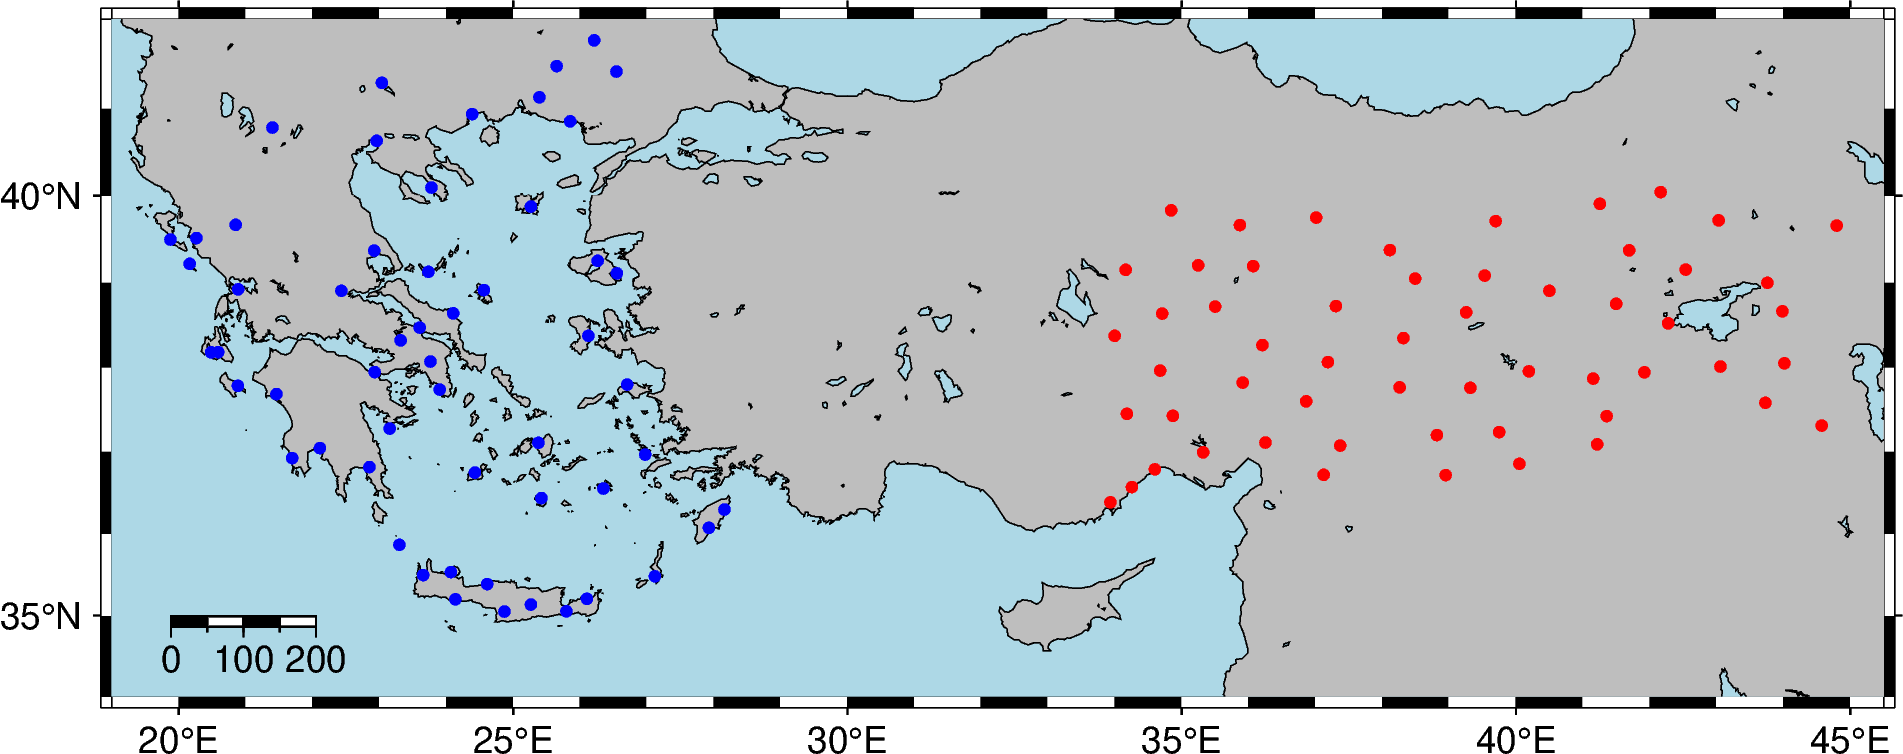
\includegraphics[width=\textwidth]{allstations.png}}
\end{minipage}

\begin{center}
\vspace*{-.1cm}
\textcolor{blue!40}{\rule{\textwidth}{1pt}}\\
{\footnotesize \textit{\textbf{Acknowledgments} to Metrica SA for the free availability of\\ the 1Hz GNSS data of HxGN SmartNet for this study, and TUSAGA-Aktif provide GNSS data of Turkish GNSS stations }}

\hspace*{.2cm}
  
\includegraphics[width=.3\textwidth]{logo_HXgn.png}~~~
  
\includegraphics[width=.2\textwidth]{logo_metrica.png}~~~
  
\includegraphics[width=.1\textwidth]{logo_hgm.png}~~~
  
\includegraphics[width=.1\textwidth]{logo_tkgm.png}
\end{center}   
\vspace*{-1.2cm}
%\textcolor{blue!40}{\rule{\textwidth}{1pt}}\\

}

%----------------------------------------------------------------------------------------
%	STRAIN ALGORITHMS
%----------------------------------------------------------------------------------------

\headerbox{GNSS Data Processing}{name=algorithms,column=1,row=0}{ 
\label{dataanalysis}
Data collected from the selected network of 95 GNSS sites were processed using the
well known PPP-AR approach, in pseudo-kinematic mode, estimating site cordinates at every measurement epoch.
Below, we summarize analysis options and products used: 

\vspace*{.1cm}
\textbf{Processing scheme:}
\begin{itemize}\setlength\itemsep{.1em}
  \item Precise Point Positioning with Ambiguity Resolution using PRIDE-PPPAR Software (v3.1.2) \cite{Geng_2019}.
  \item Satellite systems: GPS / GLO / GAL / BDS-2/3
  \item Elevation angle: 7 deg
  \item Sampling interval: 1s
  \item Coordinates estimated in pseudo-kinematic mode
  \item Reference Frame: IGS20
  \item Final IGS Products for satellite orbits and EOPs
  \item ANTEX File: IGS20\_2247
  \item Tropospheric modeling: VMF1
\end{itemize}

}

\headerbox{Time Series Analysis}{name=tsa1,column=1,row=0, below=algorithms, bottomaligned=resval}{ 
\label{tsanalysis1}


\textbf{1. Pre-processing and Filtering of GNSS Data}

Co-seismic displacements were estimated only for GNSS stations located within 800 km of the earthquake epicenters. For stations situated at distances greater than 800 km, no significant co-seismic displacements were expected.

Low-frequency noise in the GNSS data—likely caused by multipath effects, unmitigated tropospheric delays, and other sources—was suppressed using a high-pass Butterworth filter with a cut-off frequency of 0.1 Hz. This filtering effectively eliminated slow-varying noise components without significantly altering potential dynamic displacements
~\\[-.2cm]

\textbf{2. Peak Ground Displacement and Noise Estimation}

The transient seismic response window for each GNSS station was defined as starting at the arrival time of the P-waves—calculated assuming a velocity of 6 km/s—and spanning 400 seconds to ensure the full signal was captured. Peak Ground Displacement (PGD) in the NEU components was identified as the maximum value within this interval. To estimate the noise level, we calculated the standard deviation of the filtered neu time series over a 10-minute window prior to the first seismic event. A conservative threshold of 3$\sigma$ was used to distinguish real transient responses from background noise.
}
%----------------------------------------------------------------------------------------

\end{poster}

\end{document}
